
% Default to the notebook output style

    


% Inherit from the specified cell style.




    
\documentclass[11pt]{article}

    
    
    \usepackage[T1]{fontenc}
    % Nicer default font (+ math font) than Computer Modern for most use cases
    \usepackage{mathpazo}

    % Basic figure setup, for now with no caption control since it's done
    % automatically by Pandoc (which extracts ![](path) syntax from Markdown).
    \usepackage{graphicx}
    % We will generate all images so they have a width \maxwidth. This means
    % that they will get their normal width if they fit onto the page, but
    % are scaled down if they would overflow the margins.
    \makeatletter
    \def\maxwidth{\ifdim\Gin@nat@width>\linewidth\linewidth
    \else\Gin@nat@width\fi}
    \makeatother
    \let\Oldincludegraphics\includegraphics
    % Set max figure width to be 80% of text width, for now hardcoded.
    \renewcommand{\includegraphics}[1]{\Oldincludegraphics[width=.8\maxwidth]{#1}}
    % Ensure that by default, figures have no caption (until we provide a
    % proper Figure object with a Caption API and a way to capture that
    % in the conversion process - todo).
    \usepackage{caption}
    \DeclareCaptionLabelFormat{nolabel}{}
    \captionsetup{labelformat=nolabel}

    \usepackage{adjustbox} % Used to constrain images to a maximum size 
    \usepackage{xcolor} % Allow colors to be defined
    \usepackage{enumerate} % Needed for markdown enumerations to work
    \usepackage{geometry} % Used to adjust the document margins
    \usepackage{amsmath} % Equations
    \usepackage{amssymb} % Equations
    \usepackage{textcomp} % defines textquotesingle
    % Hack from http://tex.stackexchange.com/a/47451/13684:
    \AtBeginDocument{%
        \def\PYZsq{\textquotesingle}% Upright quotes in Pygmentized code
    }
    \usepackage{upquote} % Upright quotes for verbatim code
    \usepackage{eurosym} % defines \euro
    \usepackage[mathletters]{ucs} % Extended unicode (utf-8) support
    \usepackage[utf8x]{inputenc} % Allow utf-8 characters in the tex document
    \usepackage{fancyvrb} % verbatim replacement that allows latex
    \usepackage{grffile} % extends the file name processing of package graphics 
                         % to support a larger range 
    % The hyperref package gives us a pdf with properly built
    % internal navigation ('pdf bookmarks' for the table of contents,
    % internal cross-reference links, web links for URLs, etc.)
    \usepackage{hyperref}
    \usepackage{longtable} % longtable support required by pandoc >1.10
    \usepackage{booktabs}  % table support for pandoc > 1.12.2
    \usepackage[inline]{enumitem} % IRkernel/repr support (it uses the enumerate* environment)
    \usepackage[normalem]{ulem} % ulem is needed to support strikethroughs (\sout)
                                % normalem makes italics be italics, not underlines
    

    
    
    % Colors for the hyperref package
    \definecolor{urlcolor}{rgb}{0,.145,.698}
    \definecolor{linkcolor}{rgb}{.71,0.21,0.01}
    \definecolor{citecolor}{rgb}{.12,.54,.11}

    % ANSI colors
    \definecolor{ansi-black}{HTML}{3E424D}
    \definecolor{ansi-black-intense}{HTML}{282C36}
    \definecolor{ansi-red}{HTML}{E75C58}
    \definecolor{ansi-red-intense}{HTML}{B22B31}
    \definecolor{ansi-green}{HTML}{00A250}
    \definecolor{ansi-green-intense}{HTML}{007427}
    \definecolor{ansi-yellow}{HTML}{DDB62B}
    \definecolor{ansi-yellow-intense}{HTML}{B27D12}
    \definecolor{ansi-blue}{HTML}{208FFB}
    \definecolor{ansi-blue-intense}{HTML}{0065CA}
    \definecolor{ansi-magenta}{HTML}{D160C4}
    \definecolor{ansi-magenta-intense}{HTML}{A03196}
    \definecolor{ansi-cyan}{HTML}{60C6C8}
    \definecolor{ansi-cyan-intense}{HTML}{258F8F}
    \definecolor{ansi-white}{HTML}{C5C1B4}
    \definecolor{ansi-white-intense}{HTML}{A1A6B2}

    % commands and environments needed by pandoc snippets
    % extracted from the output of `pandoc -s`
    \providecommand{\tightlist}{%
      \setlength{\itemsep}{0pt}\setlength{\parskip}{0pt}}
    \DefineVerbatimEnvironment{Highlighting}{Verbatim}{commandchars=\\\{\}}
    % Add ',fontsize=\small' for more characters per line
    \newenvironment{Shaded}{}{}
    \newcommand{\KeywordTok}[1]{\textcolor[rgb]{0.00,0.44,0.13}{\textbf{{#1}}}}
    \newcommand{\DataTypeTok}[1]{\textcolor[rgb]{0.56,0.13,0.00}{{#1}}}
    \newcommand{\DecValTok}[1]{\textcolor[rgb]{0.25,0.63,0.44}{{#1}}}
    \newcommand{\BaseNTok}[1]{\textcolor[rgb]{0.25,0.63,0.44}{{#1}}}
    \newcommand{\FloatTok}[1]{\textcolor[rgb]{0.25,0.63,0.44}{{#1}}}
    \newcommand{\CharTok}[1]{\textcolor[rgb]{0.25,0.44,0.63}{{#1}}}
    \newcommand{\StringTok}[1]{\textcolor[rgb]{0.25,0.44,0.63}{{#1}}}
    \newcommand{\CommentTok}[1]{\textcolor[rgb]{0.38,0.63,0.69}{\textit{{#1}}}}
    \newcommand{\OtherTok}[1]{\textcolor[rgb]{0.00,0.44,0.13}{{#1}}}
    \newcommand{\AlertTok}[1]{\textcolor[rgb]{1.00,0.00,0.00}{\textbf{{#1}}}}
    \newcommand{\FunctionTok}[1]{\textcolor[rgb]{0.02,0.16,0.49}{{#1}}}
    \newcommand{\RegionMarkerTok}[1]{{#1}}
    \newcommand{\ErrorTok}[1]{\textcolor[rgb]{1.00,0.00,0.00}{\textbf{{#1}}}}
    \newcommand{\NormalTok}[1]{{#1}}
    
    % Additional commands for more recent versions of Pandoc
    \newcommand{\ConstantTok}[1]{\textcolor[rgb]{0.53,0.00,0.00}{{#1}}}
    \newcommand{\SpecialCharTok}[1]{\textcolor[rgb]{0.25,0.44,0.63}{{#1}}}
    \newcommand{\VerbatimStringTok}[1]{\textcolor[rgb]{0.25,0.44,0.63}{{#1}}}
    \newcommand{\SpecialStringTok}[1]{\textcolor[rgb]{0.73,0.40,0.53}{{#1}}}
    \newcommand{\ImportTok}[1]{{#1}}
    \newcommand{\DocumentationTok}[1]{\textcolor[rgb]{0.73,0.13,0.13}{\textit{{#1}}}}
    \newcommand{\AnnotationTok}[1]{\textcolor[rgb]{0.38,0.63,0.69}{\textbf{\textit{{#1}}}}}
    \newcommand{\CommentVarTok}[1]{\textcolor[rgb]{0.38,0.63,0.69}{\textbf{\textit{{#1}}}}}
    \newcommand{\VariableTok}[1]{\textcolor[rgb]{0.10,0.09,0.49}{{#1}}}
    \newcommand{\ControlFlowTok}[1]{\textcolor[rgb]{0.00,0.44,0.13}{\textbf{{#1}}}}
    \newcommand{\OperatorTok}[1]{\textcolor[rgb]{0.40,0.40,0.40}{{#1}}}
    \newcommand{\BuiltInTok}[1]{{#1}}
    \newcommand{\ExtensionTok}[1]{{#1}}
    \newcommand{\PreprocessorTok}[1]{\textcolor[rgb]{0.74,0.48,0.00}{{#1}}}
    \newcommand{\AttributeTok}[1]{\textcolor[rgb]{0.49,0.56,0.16}{{#1}}}
    \newcommand{\InformationTok}[1]{\textcolor[rgb]{0.38,0.63,0.69}{\textbf{\textit{{#1}}}}}
    \newcommand{\WarningTok}[1]{\textcolor[rgb]{0.38,0.63,0.69}{\textbf{\textit{{#1}}}}}
    
    
    % Define a nice break command that doesn't care if a line doesn't already
    % exist.
    \def\br{\hspace*{\fill} \\* }
    % Math Jax compatability definitions
    \def\gt{>}
    \def\lt{<}
    % Document parameters
    \title{notebook}
    
    
    

    % Pygments definitions
    
\makeatletter
\def\PY@reset{\let\PY@it=\relax \let\PY@bf=\relax%
    \let\PY@ul=\relax \let\PY@tc=\relax%
    \let\PY@bc=\relax \let\PY@ff=\relax}
\def\PY@tok#1{\csname PY@tok@#1\endcsname}
\def\PY@toks#1+{\ifx\relax#1\empty\else%
    \PY@tok{#1}\expandafter\PY@toks\fi}
\def\PY@do#1{\PY@bc{\PY@tc{\PY@ul{%
    \PY@it{\PY@bf{\PY@ff{#1}}}}}}}
\def\PY#1#2{\PY@reset\PY@toks#1+\relax+\PY@do{#2}}

\expandafter\def\csname PY@tok@w\endcsname{\def\PY@tc##1{\textcolor[rgb]{0.73,0.73,0.73}{##1}}}
\expandafter\def\csname PY@tok@c\endcsname{\let\PY@it=\textit\def\PY@tc##1{\textcolor[rgb]{0.25,0.50,0.50}{##1}}}
\expandafter\def\csname PY@tok@cp\endcsname{\def\PY@tc##1{\textcolor[rgb]{0.74,0.48,0.00}{##1}}}
\expandafter\def\csname PY@tok@k\endcsname{\let\PY@bf=\textbf\def\PY@tc##1{\textcolor[rgb]{0.00,0.50,0.00}{##1}}}
\expandafter\def\csname PY@tok@kp\endcsname{\def\PY@tc##1{\textcolor[rgb]{0.00,0.50,0.00}{##1}}}
\expandafter\def\csname PY@tok@kt\endcsname{\def\PY@tc##1{\textcolor[rgb]{0.69,0.00,0.25}{##1}}}
\expandafter\def\csname PY@tok@o\endcsname{\def\PY@tc##1{\textcolor[rgb]{0.40,0.40,0.40}{##1}}}
\expandafter\def\csname PY@tok@ow\endcsname{\let\PY@bf=\textbf\def\PY@tc##1{\textcolor[rgb]{0.67,0.13,1.00}{##1}}}
\expandafter\def\csname PY@tok@nb\endcsname{\def\PY@tc##1{\textcolor[rgb]{0.00,0.50,0.00}{##1}}}
\expandafter\def\csname PY@tok@nf\endcsname{\def\PY@tc##1{\textcolor[rgb]{0.00,0.00,1.00}{##1}}}
\expandafter\def\csname PY@tok@nc\endcsname{\let\PY@bf=\textbf\def\PY@tc##1{\textcolor[rgb]{0.00,0.00,1.00}{##1}}}
\expandafter\def\csname PY@tok@nn\endcsname{\let\PY@bf=\textbf\def\PY@tc##1{\textcolor[rgb]{0.00,0.00,1.00}{##1}}}
\expandafter\def\csname PY@tok@ne\endcsname{\let\PY@bf=\textbf\def\PY@tc##1{\textcolor[rgb]{0.82,0.25,0.23}{##1}}}
\expandafter\def\csname PY@tok@nv\endcsname{\def\PY@tc##1{\textcolor[rgb]{0.10,0.09,0.49}{##1}}}
\expandafter\def\csname PY@tok@no\endcsname{\def\PY@tc##1{\textcolor[rgb]{0.53,0.00,0.00}{##1}}}
\expandafter\def\csname PY@tok@nl\endcsname{\def\PY@tc##1{\textcolor[rgb]{0.63,0.63,0.00}{##1}}}
\expandafter\def\csname PY@tok@ni\endcsname{\let\PY@bf=\textbf\def\PY@tc##1{\textcolor[rgb]{0.60,0.60,0.60}{##1}}}
\expandafter\def\csname PY@tok@na\endcsname{\def\PY@tc##1{\textcolor[rgb]{0.49,0.56,0.16}{##1}}}
\expandafter\def\csname PY@tok@nt\endcsname{\let\PY@bf=\textbf\def\PY@tc##1{\textcolor[rgb]{0.00,0.50,0.00}{##1}}}
\expandafter\def\csname PY@tok@nd\endcsname{\def\PY@tc##1{\textcolor[rgb]{0.67,0.13,1.00}{##1}}}
\expandafter\def\csname PY@tok@s\endcsname{\def\PY@tc##1{\textcolor[rgb]{0.73,0.13,0.13}{##1}}}
\expandafter\def\csname PY@tok@sd\endcsname{\let\PY@it=\textit\def\PY@tc##1{\textcolor[rgb]{0.73,0.13,0.13}{##1}}}
\expandafter\def\csname PY@tok@si\endcsname{\let\PY@bf=\textbf\def\PY@tc##1{\textcolor[rgb]{0.73,0.40,0.53}{##1}}}
\expandafter\def\csname PY@tok@se\endcsname{\let\PY@bf=\textbf\def\PY@tc##1{\textcolor[rgb]{0.73,0.40,0.13}{##1}}}
\expandafter\def\csname PY@tok@sr\endcsname{\def\PY@tc##1{\textcolor[rgb]{0.73,0.40,0.53}{##1}}}
\expandafter\def\csname PY@tok@ss\endcsname{\def\PY@tc##1{\textcolor[rgb]{0.10,0.09,0.49}{##1}}}
\expandafter\def\csname PY@tok@sx\endcsname{\def\PY@tc##1{\textcolor[rgb]{0.00,0.50,0.00}{##1}}}
\expandafter\def\csname PY@tok@m\endcsname{\def\PY@tc##1{\textcolor[rgb]{0.40,0.40,0.40}{##1}}}
\expandafter\def\csname PY@tok@gh\endcsname{\let\PY@bf=\textbf\def\PY@tc##1{\textcolor[rgb]{0.00,0.00,0.50}{##1}}}
\expandafter\def\csname PY@tok@gu\endcsname{\let\PY@bf=\textbf\def\PY@tc##1{\textcolor[rgb]{0.50,0.00,0.50}{##1}}}
\expandafter\def\csname PY@tok@gd\endcsname{\def\PY@tc##1{\textcolor[rgb]{0.63,0.00,0.00}{##1}}}
\expandafter\def\csname PY@tok@gi\endcsname{\def\PY@tc##1{\textcolor[rgb]{0.00,0.63,0.00}{##1}}}
\expandafter\def\csname PY@tok@gr\endcsname{\def\PY@tc##1{\textcolor[rgb]{1.00,0.00,0.00}{##1}}}
\expandafter\def\csname PY@tok@ge\endcsname{\let\PY@it=\textit}
\expandafter\def\csname PY@tok@gs\endcsname{\let\PY@bf=\textbf}
\expandafter\def\csname PY@tok@gp\endcsname{\let\PY@bf=\textbf\def\PY@tc##1{\textcolor[rgb]{0.00,0.00,0.50}{##1}}}
\expandafter\def\csname PY@tok@go\endcsname{\def\PY@tc##1{\textcolor[rgb]{0.53,0.53,0.53}{##1}}}
\expandafter\def\csname PY@tok@gt\endcsname{\def\PY@tc##1{\textcolor[rgb]{0.00,0.27,0.87}{##1}}}
\expandafter\def\csname PY@tok@err\endcsname{\def\PY@bc##1{\setlength{\fboxsep}{0pt}\fcolorbox[rgb]{1.00,0.00,0.00}{1,1,1}{\strut ##1}}}
\expandafter\def\csname PY@tok@kc\endcsname{\let\PY@bf=\textbf\def\PY@tc##1{\textcolor[rgb]{0.00,0.50,0.00}{##1}}}
\expandafter\def\csname PY@tok@kd\endcsname{\let\PY@bf=\textbf\def\PY@tc##1{\textcolor[rgb]{0.00,0.50,0.00}{##1}}}
\expandafter\def\csname PY@tok@kn\endcsname{\let\PY@bf=\textbf\def\PY@tc##1{\textcolor[rgb]{0.00,0.50,0.00}{##1}}}
\expandafter\def\csname PY@tok@kr\endcsname{\let\PY@bf=\textbf\def\PY@tc##1{\textcolor[rgb]{0.00,0.50,0.00}{##1}}}
\expandafter\def\csname PY@tok@bp\endcsname{\def\PY@tc##1{\textcolor[rgb]{0.00,0.50,0.00}{##1}}}
\expandafter\def\csname PY@tok@fm\endcsname{\def\PY@tc##1{\textcolor[rgb]{0.00,0.00,1.00}{##1}}}
\expandafter\def\csname PY@tok@vc\endcsname{\def\PY@tc##1{\textcolor[rgb]{0.10,0.09,0.49}{##1}}}
\expandafter\def\csname PY@tok@vg\endcsname{\def\PY@tc##1{\textcolor[rgb]{0.10,0.09,0.49}{##1}}}
\expandafter\def\csname PY@tok@vi\endcsname{\def\PY@tc##1{\textcolor[rgb]{0.10,0.09,0.49}{##1}}}
\expandafter\def\csname PY@tok@vm\endcsname{\def\PY@tc##1{\textcolor[rgb]{0.10,0.09,0.49}{##1}}}
\expandafter\def\csname PY@tok@sa\endcsname{\def\PY@tc##1{\textcolor[rgb]{0.73,0.13,0.13}{##1}}}
\expandafter\def\csname PY@tok@sb\endcsname{\def\PY@tc##1{\textcolor[rgb]{0.73,0.13,0.13}{##1}}}
\expandafter\def\csname PY@tok@sc\endcsname{\def\PY@tc##1{\textcolor[rgb]{0.73,0.13,0.13}{##1}}}
\expandafter\def\csname PY@tok@dl\endcsname{\def\PY@tc##1{\textcolor[rgb]{0.73,0.13,0.13}{##1}}}
\expandafter\def\csname PY@tok@s2\endcsname{\def\PY@tc##1{\textcolor[rgb]{0.73,0.13,0.13}{##1}}}
\expandafter\def\csname PY@tok@sh\endcsname{\def\PY@tc##1{\textcolor[rgb]{0.73,0.13,0.13}{##1}}}
\expandafter\def\csname PY@tok@s1\endcsname{\def\PY@tc##1{\textcolor[rgb]{0.73,0.13,0.13}{##1}}}
\expandafter\def\csname PY@tok@mb\endcsname{\def\PY@tc##1{\textcolor[rgb]{0.40,0.40,0.40}{##1}}}
\expandafter\def\csname PY@tok@mf\endcsname{\def\PY@tc##1{\textcolor[rgb]{0.40,0.40,0.40}{##1}}}
\expandafter\def\csname PY@tok@mh\endcsname{\def\PY@tc##1{\textcolor[rgb]{0.40,0.40,0.40}{##1}}}
\expandafter\def\csname PY@tok@mi\endcsname{\def\PY@tc##1{\textcolor[rgb]{0.40,0.40,0.40}{##1}}}
\expandafter\def\csname PY@tok@il\endcsname{\def\PY@tc##1{\textcolor[rgb]{0.40,0.40,0.40}{##1}}}
\expandafter\def\csname PY@tok@mo\endcsname{\def\PY@tc##1{\textcolor[rgb]{0.40,0.40,0.40}{##1}}}
\expandafter\def\csname PY@tok@ch\endcsname{\let\PY@it=\textit\def\PY@tc##1{\textcolor[rgb]{0.25,0.50,0.50}{##1}}}
\expandafter\def\csname PY@tok@cm\endcsname{\let\PY@it=\textit\def\PY@tc##1{\textcolor[rgb]{0.25,0.50,0.50}{##1}}}
\expandafter\def\csname PY@tok@cpf\endcsname{\let\PY@it=\textit\def\PY@tc##1{\textcolor[rgb]{0.25,0.50,0.50}{##1}}}
\expandafter\def\csname PY@tok@c1\endcsname{\let\PY@it=\textit\def\PY@tc##1{\textcolor[rgb]{0.25,0.50,0.50}{##1}}}
\expandafter\def\csname PY@tok@cs\endcsname{\let\PY@it=\textit\def\PY@tc##1{\textcolor[rgb]{0.25,0.50,0.50}{##1}}}

\def\PYZbs{\char`\\}
\def\PYZus{\char`\_}
\def\PYZob{\char`\{}
\def\PYZcb{\char`\}}
\def\PYZca{\char`\^}
\def\PYZam{\char`\&}
\def\PYZlt{\char`\<}
\def\PYZgt{\char`\>}
\def\PYZsh{\char`\#}
\def\PYZpc{\char`\%}
\def\PYZdl{\char`\$}
\def\PYZhy{\char`\-}
\def\PYZsq{\char`\'}
\def\PYZdq{\char`\"}
\def\PYZti{\char`\~}
% for compatibility with earlier versions
\def\PYZat{@}
\def\PYZlb{[}
\def\PYZrb{]}
\makeatother


    % Exact colors from NB
    \definecolor{incolor}{rgb}{0.0, 0.0, 0.5}
    \definecolor{outcolor}{rgb}{0.545, 0.0, 0.0}



    
    % Prevent overflowing lines due to hard-to-break entities
    \sloppy 
    % Setup hyperref package
    \hypersetup{
      breaklinks=true,  % so long urls are correctly broken across lines
      colorlinks=true,
      urlcolor=urlcolor,
      linkcolor=linkcolor,
      citecolor=citecolor,
      }
    % Slightly bigger margins than the latex defaults
    
    \geometry{verbose,tmargin=1in,bmargin=1in,lmargin=1in,rmargin=1in}
    
    

    \begin{document}
    
    
    \maketitle
    
    

    
    \section{A journey into Convolutional Neural Network
visualisation}\label{a-journey-into-convolutional-neural-network-visualisation}

There is one famous urban legend about computer vision. Around the 80s,
the US military wanted to use neural networks to automatically detect
camouflaged enemy tanks. They took a number of pictures of trees without
tanks and then pictures with the same trees with tanks behind them. The
results were impressive. So impressive that the army wanted to be sure
the net had correctly generalized. They took new pictures of woods with
and without tanks and they showed them again to the network. This time,
the model performed terribly, it was not able to discriminate between
pictures tanks behind woods and just trees. It turned out, that all the
pictures with of plain woods were taken on a cloudy day while the ones
with tanks on a sunny day! In reality, the network lean to recognize the
weather, not the enemy tanks.

With this article, we are going to see different techniques to
\emph{understand} what it is going on inside a Convolutional Neural
Network to avoid making the same US' army mistake.

We are going to use \href{https://pytorch.org/}{Pytorch}. All the code
can be found
\href{https://github.com/FrancescoSaverioZuppichini/A-journey-into-Convolutional-Neural-Network-visualization-}{here}.
Most of the visualizations were developed from scratch, however, some
inspiration and parts were taken from
\href{https://github.com/utkuozbulak/pytorch-cnn-visualizations/tree/master/src}{here}

We will first introduce each technique by briefly explain it and making
some example and comparison between different classic computer vision
models, \texttt{alexnet}, \texttt{vgg16} and \texttt{resnet}. Then we
will try to better understand a model used in robotics to avoid
obstacles using frontal camera's images.

Our goal is not to explain in detail how each technique works, even if
some of them are very simple since this is already done by each paper.
But to use them to help the reader visualize different model with
different inputs to better understand and highlight what and how
different models see an input. For example, we will see with features in
the input image is used to understand that it contains a cat.

    \section{Preambula}\label{preambula}

Let's start our journey by selecting some images to be used as inputs.
We are first going to fire up \texttt{alexnet} to start exploring the
first technique.

    \begin{Verbatim}[commandchars=\\\{\}]
{\color{incolor}In [{\color{incolor}85}]:} \PY{k+kn}{from} \PY{n+nn}{torchvision}\PY{n+nn}{.}\PY{n+nn}{models} \PY{k}{import} \PY{o}{*}
         
         \PY{n}{model} \PY{o}{=} \PY{n}{alexnet}\PY{p}{(}\PY{n}{pretrained}\PY{o}{=}\PY{k+kc}{True}\PY{p}{)}
         \PY{n+nb}{print}\PY{p}{(}\PY{n}{model}\PY{p}{)}
\end{Verbatim}


    \begin{Verbatim}[commandchars=\\\{\}]
AlexNet(
  (features): Sequential(
    (0): Conv2d(3, 64, kernel\_size=(11, 11), stride=(4, 4), padding=(2, 2))
    (1): ReLU(inplace)
    (2): MaxPool2d(kernel\_size=3, stride=2, padding=0, dilation=1, ceil\_mode=False)
    (3): Conv2d(64, 192, kernel\_size=(5, 5), stride=(1, 1), padding=(2, 2))
    (4): ReLU(inplace)
    (5): MaxPool2d(kernel\_size=3, stride=2, padding=0, dilation=1, ceil\_mode=False)
    (6): Conv2d(192, 384, kernel\_size=(3, 3), stride=(1, 1), padding=(1, 1))
    (7): ReLU(inplace)
    (8): Conv2d(384, 256, kernel\_size=(3, 3), stride=(1, 1), padding=(1, 1))
    (9): ReLU(inplace)
    (10): Conv2d(256, 256, kernel\_size=(3, 3), stride=(1, 1), padding=(1, 1))
    (11): ReLU(inplace)
    (12): MaxPool2d(kernel\_size=3, stride=2, padding=0, dilation=1, ceil\_mode=False)
  )
  (classifier): Sequential(
    (0): Dropout(p=0.5)
    (1): Linear(in\_features=9216, out\_features=4096, bias=True)
    (2): ReLU(inplace)
    (3): Dropout(p=0.5)
    (4): Linear(in\_features=4096, out\_features=4096, bias=True)
    (5): ReLU(inplace)
    (6): Linear(in\_features=4096, out\_features=1000, bias=True)
  )
)

    \end{Verbatim}

    Now we need some inputs

    \begin{Verbatim}[commandchars=\\\{\}]
{\color{incolor}In [{\color{incolor}26}]:} \PY{o}{\PYZpc{}}\PY{k}{matplotlib} notebook
\end{Verbatim}


    \begin{Verbatim}[commandchars=\\\{\}]
{\color{incolor}In [{\color{incolor}27}]:} \PY{k+kn}{import} \PY{n+nn}{glob}
         \PY{k+kn}{import} \PY{n+nn}{matplotlib}\PY{n+nn}{.}\PY{n+nn}{pyplot} \PY{k}{as} \PY{n+nn}{plt}
         \PY{k+kn}{import} \PY{n+nn}{numpy} \PY{k}{as} \PY{n+nn}{np}
         \PY{k+kn}{import} \PY{n+nn}{torch} 
         
         \PY{k+kn}{from} \PY{n+nn}{PIL} \PY{k}{import} \PY{n}{Image}
         
         \PY{n}{plt}\PY{o}{.}\PY{n}{rcParams}\PY{p}{[}\PY{l+s+s2}{\PYZdq{}}\PY{l+s+s2}{figure.figsize}\PY{l+s+s2}{\PYZdq{}}\PY{p}{]}\PY{o}{=}\PY{l+m+mi}{7}\PY{p}{,}\PY{l+m+mi}{7}
\end{Verbatim}


    \begin{Verbatim}[commandchars=\\\{\}]
{\color{incolor}In [{\color{incolor}28}]:} \PY{k}{def} \PY{n+nf}{tensor2img}\PY{p}{(}\PY{n}{tensor}\PY{p}{,} \PY{n}{ax}\PY{o}{=}\PY{n}{plt}\PY{p}{)}\PY{p}{:}
             \PY{n}{tensor} \PY{o}{=} \PY{n}{tensor}\PY{o}{.}\PY{n}{squeeze}\PY{p}{(}\PY{p}{)}
             \PY{k}{if} \PY{n+nb}{len}\PY{p}{(}\PY{n}{tensor}\PY{o}{.}\PY{n}{shape}\PY{p}{)} \PY{o}{\PYZgt{}} \PY{l+m+mi}{2}\PY{p}{:} \PY{n}{tensor} \PY{o}{=} \PY{n}{tensor}\PY{o}{.}\PY{n}{permute}\PY{p}{(}\PY{l+m+mi}{1}\PY{p}{,} \PY{l+m+mi}{2}\PY{p}{,} \PY{l+m+mi}{0}\PY{p}{)}
             \PY{n}{img} \PY{o}{=} \PY{n}{tensor}\PY{o}{.}\PY{n}{detach}\PY{p}{(}\PY{p}{)}\PY{o}{.}\PY{n}{cpu}\PY{p}{(}\PY{p}{)}\PY{o}{.}\PY{n}{numpy}\PY{p}{(}\PY{p}{)}
             \PY{k}{return} \PY{n}{img}
\end{Verbatim}


    \begin{Verbatim}[commandchars=\\\{\}]
{\color{incolor}In [{\color{incolor}29}]:} \PY{k}{def} \PY{n+nf}{subplot}\PY{p}{(}\PY{n}{images}\PY{p}{,} \PY{n}{parse}\PY{o}{=}\PY{k}{lambda} \PY{n}{x}\PY{p}{:} \PY{n}{x}\PY{p}{,} \PY{n}{rows\PYZus{}titles}\PY{o}{=}\PY{k+kc}{None}\PY{p}{,} \PY{n}{cols\PYZus{}titles}\PY{o}{=}\PY{k+kc}{None}\PY{p}{,} \PY{n}{title}\PY{o}{=}\PY{l+s+s1}{\PYZsq{}}\PY{l+s+s1}{\PYZsq{}}\PY{p}{,} \PY{o}{*}\PY{n}{args}\PY{p}{,} \PY{o}{*}\PY{o}{*}\PY{n}{kwargs}\PY{p}{)}\PY{p}{:}
             \PY{n}{fig}\PY{p}{,} \PY{n}{ax} \PY{o}{=} \PY{n}{plt}\PY{o}{.}\PY{n}{subplots}\PY{p}{(}\PY{o}{*}\PY{n}{args}\PY{p}{,} \PY{o}{*}\PY{o}{*}\PY{n}{kwargs}\PY{p}{)}
             \PY{n}{fig}\PY{o}{.}\PY{n}{suptitle}\PY{p}{(}\PY{n}{title}\PY{p}{)}
             \PY{n}{i} \PY{o}{=} \PY{l+m+mi}{0}
             \PY{k}{try}\PY{p}{:}
                 \PY{k}{for} \PY{n}{row} \PY{o+ow}{in} \PY{n}{ax}\PY{p}{:}
                     \PY{k}{if} \PY{n}{rows\PYZus{}titles} \PY{o+ow}{is} \PY{o+ow}{not} \PY{k+kc}{None}\PY{p}{:} \PY{n}{row}\PY{o}{.}\PY{n}{set\PYZus{}title}\PY{p}{(}\PY{n}{rows\PYZus{}titles}\PY{p}{[}\PY{n}{i}\PY{p}{]}\PY{p}{)}
                     \PY{k}{try}\PY{p}{:}
                         \PY{k}{for} \PY{n}{j}\PY{p}{,}\PY{n}{col} \PY{o+ow}{in} \PY{n+nb}{enumerate}\PY{p}{(}\PY{n}{row}\PY{p}{)}\PY{p}{:}
                             \PY{k}{if} \PY{n}{cols\PYZus{}titles} \PY{o+ow}{is} \PY{o+ow}{not} \PY{k+kc}{None}\PY{p}{:}  \PY{n}{col}\PY{o}{.}\PY{n}{set\PYZus{}title}\PY{p}{(}\PY{n}{cols\PYZus{}titles}\PY{p}{[}\PY{n}{j}\PY{p}{]}\PY{p}{)}
                             \PY{n}{col}\PY{o}{.}\PY{n}{imshow}\PY{p}{(}\PY{n}{parse}\PY{p}{(}\PY{n}{images}\PY{p}{[}\PY{n}{i}\PY{p}{]}\PY{p}{)}\PY{p}{)}
                             \PY{n}{col}\PY{o}{.}\PY{n}{axis}\PY{p}{(}\PY{l+s+s1}{\PYZsq{}}\PY{l+s+s1}{off}\PY{l+s+s1}{\PYZsq{}}\PY{p}{)}
                             \PY{n}{col}\PY{o}{.}\PY{n}{set\PYZus{}aspect}\PY{p}{(}\PY{l+s+s1}{\PYZsq{}}\PY{l+s+s1}{equal}\PY{l+s+s1}{\PYZsq{}}\PY{p}{)}
                             \PY{n}{i} \PY{o}{+}\PY{o}{=} \PY{l+m+mi}{1}
                     \PY{k}{except} \PY{n+ne}{TypeError}\PY{p}{:}
                         \PY{n}{row}\PY{o}{.}\PY{n}{imshow}\PY{p}{(}\PY{n}{parse}\PY{p}{(}\PY{n}{images}\PY{p}{[}\PY{n}{i}\PY{p}{]}\PY{p}{)}\PY{p}{)}
                         \PY{n}{row}\PY{o}{.}\PY{n}{axis}\PY{p}{(}\PY{l+s+s1}{\PYZsq{}}\PY{l+s+s1}{off}\PY{l+s+s1}{\PYZsq{}}\PY{p}{)}
                         \PY{n}{row}\PY{o}{.}\PY{n}{set\PYZus{}aspect}\PY{p}{(}\PY{l+s+s1}{\PYZsq{}}\PY{l+s+s1}{equal}\PY{l+s+s1}{\PYZsq{}}\PY{p}{)}
                         \PY{n}{i} \PY{o}{+}\PY{o}{=} \PY{l+m+mi}{1}
                     \PY{k}{except} \PY{n+ne}{IndexError}\PY{p}{:}
                         \PY{k}{break}
             \PY{k}{except}\PY{p}{:}
                 \PY{n}{ax}\PY{o}{.}\PY{n}{imshow}\PY{p}{(}\PY{n}{parse}\PY{p}{(}\PY{n}{images}\PY{p}{[}\PY{n}{i}\PY{p}{]}\PY{p}{)}\PY{p}{)}
                 \PY{n}{ax}\PY{o}{.}\PY{n}{axis}\PY{p}{(}\PY{l+s+s1}{\PYZsq{}}\PY{l+s+s1}{off}\PY{l+s+s1}{\PYZsq{}}\PY{p}{)}
                 \PY{n}{ax}\PY{o}{.}\PY{n}{set\PYZus{}aspect}\PY{p}{(}\PY{l+s+s1}{\PYZsq{}}\PY{l+s+s1}{equal}\PY{l+s+s1}{\PYZsq{}}\PY{p}{)}
             \PY{n}{plt}\PY{o}{.}\PY{n}{subplots\PYZus{}adjust}\PY{p}{(}\PY{n}{wspace}\PY{o}{=}\PY{l+m+mi}{0}\PY{p}{,} \PY{n}{hspace}\PY{o}{=}\PY{l+m+mi}{0}\PY{p}{)}
\end{Verbatim}


    \begin{Verbatim}[commandchars=\\\{\}]
{\color{incolor}In [{\color{incolor}49}]:} \PY{k+kn}{import} \PY{n+nn}{glob}
         \PY{k+kn}{import} \PY{n+nn}{matplotlib}\PY{n+nn}{.}\PY{n+nn}{pyplot} \PY{k}{as} \PY{n+nn}{plt}
         \PY{k+kn}{import} \PY{n+nn}{numpy} \PY{k}{as} \PY{n+nn}{np}
         
         \PY{k+kn}{from} \PY{n+nn}{PIL} \PY{k}{import} \PY{n}{Image}
         
         \PY{n}{image\PYZus{}paths} \PY{o}{=} \PY{n}{glob}\PY{o}{.}\PY{n}{glob}\PY{p}{(}\PY{l+s+s1}{\PYZsq{}}\PY{l+s+s1}{./images/*.*}\PY{l+s+s1}{\PYZsq{}}\PY{p}{)}
         
         \PY{n}{images} \PY{o}{=} \PY{n+nb}{list}\PY{p}{(}\PY{n+nb}{map}\PY{p}{(}\PY{k}{lambda} \PY{n}{x}\PY{p}{:} \PY{n}{Image}\PY{o}{.}\PY{n}{open}\PY{p}{(}\PY{n}{x}\PY{p}{)}\PY{p}{,} \PY{n}{image\PYZus{}paths}\PY{p}{)}\PY{p}{)}
         
         \PY{n}{subplot}\PY{p}{(}\PY{n}{images}\PY{p}{,} \PY{n}{title}\PY{o}{=}\PY{l+s+s1}{\PYZsq{}}\PY{l+s+s1}{inputs}\PY{l+s+s1}{\PYZsq{}}\PY{p}{,} \PY{n}{rows\PYZus{}titles}\PY{o}{=}\PY{p}{[}\PY{l+s+s1}{\PYZsq{}}\PY{l+s+s1}{dog\PYZus{}cat}\PY{l+s+s1}{\PYZsq{}}\PY{p}{,}\PY{l+s+s1}{\PYZsq{}}\PY{l+s+s1}{san pietro}\PY{l+s+s1}{\PYZsq{}}\PY{p}{,}\PY{l+s+s1}{\PYZsq{}}\PY{l+s+s1}{cat}\PY{l+s+s1}{\PYZsq{}}\PY{p}{]}\PY{p}{,} \PY{n}{nrows}\PY{o}{=}\PY{l+m+mi}{1}\PY{p}{,} \PY{n}{ncols}\PY{o}{=}\PY{l+m+mi}{3}\PY{p}{)}
         
         \PY{n}{plt}\PY{o}{.}\PY{n}{show}\PY{p}{(}\PY{p}{)}
\end{Verbatim}


    
    \begin{verbatim}
<IPython.core.display.Javascript object>
    \end{verbatim}

    
    
    \begin{verbatim}
<IPython.core.display.HTML object>
    \end{verbatim}

    
    As inputs we are going to use an image with two classes, \texttt{dog}
and \texttt{cat}, the beautiful Basilica of San Pietro and a
\texttt{cat}. We know need to parse them and preprocess by normalize
them since all of our models were trained on
\href{http://www.image-net.org/}{imagenet} a huge dataset with
\texttt{1000} different classes.

    \begin{Verbatim}[commandchars=\\\{\}]
{\color{incolor}In [{\color{incolor}50}]:} \PY{k+kn}{from} \PY{n+nn}{torchvision}\PY{n+nn}{.}\PY{n+nn}{transforms} \PY{k}{import} \PY{n}{ToTensor}\PY{p}{,} \PY{n}{Resize}\PY{p}{,} \PY{n}{Compose}
         \PY{k+kn}{from} \PY{n+nn}{visualisation}\PY{n+nn}{.}\PY{n+nn}{core} \PY{k}{import} \PY{o}{*}
         \PY{k+kn}{from} \PY{n+nn}{visualisation}\PY{n+nn}{.}\PY{n+nn}{core}\PY{n+nn}{.}\PY{n+nn}{utils} \PY{k}{import} \PY{n}{image\PYZus{}net\PYZus{}preprocessing}
         
         \PY{n}{inputs}  \PY{o}{=} \PY{p}{[}\PY{n}{Compose}\PY{p}{(}\PY{p}{[}\PY{n}{Resize}\PY{p}{(}\PY{p}{(}\PY{l+m+mi}{224}\PY{p}{,}\PY{l+m+mi}{224}\PY{p}{)}\PY{p}{)}\PY{p}{,} \PY{n}{ToTensor}\PY{p}{(}\PY{p}{)}\PY{p}{,} \PY{n}{image\PYZus{}net\PYZus{}preprocessing}\PY{p}{]}\PY{p}{)}\PY{p}{(}\PY{n}{x}\PY{p}{)}\PY{o}{.}\PY{n}{unsqueeze}\PY{p}{(}\PY{l+m+mi}{0}\PY{p}{)} \PY{k}{for} \PY{n}{x} \PY{o+ow}{in} \PY{n}{images}\PY{p}{]}  \PY{c+c1}{\PYZsh{} add 1 dim for batch}
\end{Verbatim}


    We will also need the human readable label for each class

    \begin{Verbatim}[commandchars=\\\{\}]
{\color{incolor}In [{\color{incolor}86}]:} \PY{n}{imagenet2human} \PY{o}{=} \PY{p}{\PYZob{}}\PY{p}{\PYZcb{}}
         \PY{k}{with} \PY{n+nb}{open}\PY{p}{(}\PY{l+s+s1}{\PYZsq{}}\PY{l+s+s1}{imaganet2human.txt}\PY{l+s+s1}{\PYZsq{}}\PY{p}{)} \PY{k}{as} \PY{n}{f}\PY{p}{:}
             \PY{k}{for} \PY{n}{line} \PY{o+ow}{in} \PY{n}{f}\PY{o}{.}\PY{n}{readlines}\PY{p}{(}\PY{p}{)}\PY{p}{:}
                 \PY{n}{key}\PY{p}{,} \PY{n}{value} \PY{o}{=} \PY{n}{line}\PY{o}{.}\PY{n}{split}\PY{p}{(}\PY{l+s+s1}{\PYZsq{}}\PY{l+s+s1}{:}\PY{l+s+s1}{\PYZsq{}}\PY{p}{)}
                 \PY{n}{key} \PY{o}{=} \PY{n}{key}\PY{o}{.}\PY{n}{replace}\PY{p}{(}\PY{l+s+s1}{\PYZsq{}}\PY{l+s+s1}{\PYZob{}}\PY{l+s+s1}{\PYZsq{}}\PY{p}{,} \PY{l+s+s1}{\PYZsq{}}\PY{l+s+s1}{\PYZsq{}}\PY{p}{)}\PY{o}{.}\PY{n}{replace}\PY{p}{(}\PY{l+s+s1}{\PYZsq{}}\PY{l+s+s1}{\PYZcb{}}\PY{l+s+s1}{\PYZsq{}}\PY{p}{,} \PY{l+s+s1}{\PYZsq{}}\PY{l+s+s1}{\PYZsq{}}\PY{p}{)} \PY{c+c1}{\PYZsh{} I forget how regex works :) }
                 \PY{n}{value} \PY{o}{=} \PY{n}{value}\PY{o}{.}\PY{n}{replace}\PY{p}{(}\PY{l+s+s2}{\PYZdq{}}\PY{l+s+s2}{\PYZsq{}}\PY{l+s+s2}{\PYZdq{}}\PY{p}{,} \PY{l+s+s1}{\PYZsq{}}\PY{l+s+s1}{\PYZsq{}}\PY{p}{)}\PY{o}{.}\PY{n}{replace}\PY{p}{(}\PY{l+s+s2}{\PYZdq{}}\PY{l+s+s2}{,}\PY{l+s+s2}{\PYZdq{}}\PY{p}{,} \PY{l+s+s1}{\PYZsq{}}\PY{l+s+s1}{\PYZsq{}}\PY{p}{)}
                 \PY{n}{imagenet2human}\PY{p}{[}\PY{n+nb}{int}\PY{p}{(}\PY{n}{key}\PY{o}{.}\PY{n}{strip}\PY{p}{(}\PY{p}{)}\PY{p}{)}\PY{p}{]} \PY{o}{=} \PY{n+nb}{str}\PY{p}{(}\PY{n}{value}\PY{o}{.}\PY{n}{strip}\PY{p}{(}\PY{p}{)}\PY{p}{)}
                 
         \PY{n}{imagenet2human}
\end{Verbatim}


\begin{Verbatim}[commandchars=\\\{\}]
{\color{outcolor}Out[{\color{outcolor}86}]:} \{0: 'tench Tinca tinca',
          1: 'goldfish Carassius auratus',
          2: 'great white shark white shark man-eater man-eating shark Carcharodon carcharias',
          3: 'tiger shark Galeocerdo cuvieri',
          4: 'hammerhead hammerhead shark',
          5: 'electric ray crampfish numbfish torpedo',
          6: 'stingray',
          7: 'cock',
          8: 'hen',
          9: 'ostrich Struthio camelus',
          10: 'brambling Fringilla montifringilla',
          11: 'goldfinch Carduelis carduelis',
          12: 'house finch linnet Carpodacus mexicanus',
          13: 'junco snowbird',
          14: 'indigo bunting indigo finch indigo bird Passerina cyanea',
          15: 'robin American robin Turdus migratorius',
          16: 'bulbul',
          17: 'jay',
          18: 'magpie',
          19: 'chickadee',
          20: 'water ouzel dipper',
          21: 'kite',
          22: 'bald eagle American eagle Haliaeetus leucocephalus',
          23: 'vulture',
          24: 'great grey owl great gray owl Strix nebulosa',
          25: 'European fire salamander Salamandra salamandra',
          26: 'common newt Triturus vulgaris',
          27: 'eft',
          28: 'spotted salamander Ambystoma maculatum',
          29: 'axolotl mud puppy Ambystoma mexicanum',
          30: 'bullfrog Rana catesbeiana',
          31: 'tree frog tree-frog',
          32: 'tailed frog bell toad ribbed toad tailed toad Ascaphus trui',
          33: 'loggerhead loggerhead turtle Caretta caretta',
          34: 'leatherback turtle leatherback leathery turtle Dermochelys coriacea',
          35: 'mud turtle',
          36: 'terrapin',
          37: 'box turtle box tortoise',
          38: 'banded gecko',
          39: 'common iguana iguana Iguana iguana',
          40: 'American chameleon anole Anolis carolinensis',
          41: 'whiptail whiptail lizard',
          42: 'agama',
          43: 'frilled lizard Chlamydosaurus kingi',
          44: 'alligator lizard',
          45: 'Gila monster Heloderma suspectum',
          46: 'green lizard Lacerta viridis',
          47: 'African chameleon Chamaeleo chamaeleon',
          48: 'Komodo dragon Komodo lizard dragon lizard giant lizard Varanus komodoensis',
          49: 'African crocodile Nile crocodile Crocodylus niloticus',
          50: 'American alligator Alligator mississipiensis',
          51: 'triceratops',
          52: 'thunder snake worm snake Carphophis amoenus',
          53: 'ringneck snake ring-necked snake ring snake',
          54: 'hognose snake puff adder sand viper',
          55: 'green snake grass snake',
          56: 'king snake kingsnake',
          57: 'garter snake grass snake',
          58: 'water snake',
          59: 'vine snake',
          60: 'night snake Hypsiglena torquata',
          61: 'boa constrictor Constrictor constrictor',
          62: 'rock python rock snake Python sebae',
          63: 'Indian cobra Naja naja',
          64: 'green mamba',
          65: 'sea snake',
          66: 'horned viper cerastes sand viper horned asp Cerastes cornutus',
          67: 'diamondback diamondback rattlesnake Crotalus adamanteus',
          68: 'sidewinder horned rattlesnake Crotalus cerastes',
          69: 'trilobite',
          70: 'harvestman daddy longlegs Phalangium opilio',
          71: 'scorpion',
          72: 'black and gold garden spider Argiope aurantia',
          73: 'barn spider Araneus cavaticus',
          74: 'garden spider Aranea diademata',
          75: 'black widow Latrodectus mactans',
          76: 'tarantula',
          77: 'wolf spider hunting spider',
          78: 'tick',
          79: 'centipede',
          80: 'black grouse',
          81: 'ptarmigan',
          82: 'ruffed grouse partridge Bonasa umbellus',
          83: 'prairie chicken prairie grouse prairie fowl',
          84: 'peacock',
          85: 'quail',
          86: 'partridge',
          87: 'African grey African gray Psittacus erithacus',
          88: 'macaw',
          89: 'sulphur-crested cockatoo Kakatoe galerita Cacatua galerita',
          90: 'lorikeet',
          91: 'coucal',
          92: 'bee eater',
          93: 'hornbill',
          94: 'hummingbird',
          95: 'jacamar',
          96: 'toucan',
          97: 'drake',
          98: 'red-breasted merganser Mergus serrator',
          99: 'goose',
          100: 'black swan Cygnus atratus',
          101: 'tusker',
          102: 'echidna spiny anteater anteater',
          103: 'platypus duckbill duckbilled platypus duck-billed platypus Ornithorhynchus anatinus',
          104: 'wallaby brush kangaroo',
          105: 'koala koala bear kangaroo bear native bear Phascolarctos cinereus',
          106: 'wombat',
          107: 'jellyfish',
          108: 'sea anemone anemone',
          109: 'brain coral',
          110: 'flatworm platyhelminth',
          111: 'nematode nematode worm roundworm',
          112: 'conch',
          113: 'snail',
          114: 'slug',
          115: 'sea slug nudibranch',
          116: 'chiton coat-of-mail shell sea cradle polyplacophore',
          117: 'chambered nautilus pearly nautilus nautilus',
          118: 'Dungeness crab Cancer magister',
          119: 'rock crab Cancer irroratus',
          120: 'fiddler crab',
          121: 'king crab Alaska crab Alaskan king crab Alaska king crab Paralithodes camtschatica',
          122: 'American lobster Northern lobster Maine lobster Homarus americanus',
          123: 'spiny lobster langouste rock lobster crawfish crayfish sea crawfish',
          124: 'crayfish crawfish crawdad crawdaddy',
          125: 'hermit crab',
          126: 'isopod',
          127: 'white stork Ciconia ciconia',
          128: 'black stork Ciconia nigra',
          129: 'spoonbill',
          130: 'flamingo',
          131: 'little blue heron Egretta caerulea',
          132: 'American egret great white heron Egretta albus',
          133: 'bittern',
          134: 'crane',
          135: 'limpkin Aramus pictus',
          136: 'European gallinule Porphyrio porphyrio',
          137: 'American coot marsh hen mud hen water hen Fulica americana',
          138: 'bustard',
          139: 'ruddy turnstone Arenaria interpres',
          140: 'red-backed sandpiper dunlin Erolia alpina',
          141: 'redshank Tringa totanus',
          142: 'dowitcher',
          143: 'oystercatcher oyster catcher',
          144: 'pelican',
          145: 'king penguin Aptenodytes patagonica',
          146: 'albatross mollymawk',
          147: 'grey whale gray whale devilfish Eschrichtius gibbosus Eschrichtius robustus',
          148: 'killer whale killer orca grampus sea wolf Orcinus orca',
          149: 'dugong Dugong dugon',
          150: 'sea lion',
          151: 'Chihuahua',
          152: 'Japanese spaniel',
          153: 'Maltese dog Maltese terrier Maltese',
          154: 'Pekinese Pekingese Peke',
          155: 'Shih-Tzu',
          156: 'Blenheim spaniel',
          157: 'papillon',
          158: 'toy terrier',
          159: 'Rhodesian ridgeback',
          160: 'Afghan hound Afghan',
          161: 'basset basset hound',
          162: 'beagle',
          163: 'bloodhound sleuthhound',
          164: 'bluetick',
          165: 'black-and-tan coonhound',
          166: 'Walker hound Walker foxhound',
          167: 'English foxhound',
          168: 'redbone',
          169: 'borzoi Russian wolfhound',
          170: 'Irish wolfhound',
          171: 'Italian greyhound',
          172: 'whippet',
          173: 'Ibizan hound Ibizan Podenco',
          174: 'Norwegian elkhound elkhound',
          175: 'otterhound otter hound',
          176: 'Saluki gazelle hound',
          177: 'Scottish deerhound deerhound',
          178: 'Weimaraner',
          179: 'Staffordshire bullterrier Staffordshire bull terrier',
          180: 'American Staffordshire terrier Staffordshire terrier American pit bull terrier pit bull terrier',
          181: 'Bedlington terrier',
          182: 'Border terrier',
          183: 'Kerry blue terrier',
          184: 'Irish terrier',
          185: 'Norfolk terrier',
          186: 'Norwich terrier',
          187: 'Yorkshire terrier',
          188: 'wire-haired fox terrier',
          189: 'Lakeland terrier',
          190: 'Sealyham terrier Sealyham',
          191: 'Airedale Airedale terrier',
          192: 'cairn cairn terrier',
          193: 'Australian terrier',
          194: 'Dandie Dinmont Dandie Dinmont terrier',
          195: 'Boston bull Boston terrier',
          196: 'miniature schnauzer',
          197: 'giant schnauzer',
          198: 'standard schnauzer',
          199: 'Scotch terrier Scottish terrier Scottie',
          200: 'Tibetan terrier chrysanthemum dog',
          201: 'silky terrier Sydney silky',
          202: 'soft-coated wheaten terrier',
          203: 'West Highland white terrier',
          204: 'Lhasa Lhasa apso',
          205: 'flat-coated retriever',
          206: 'curly-coated retriever',
          207: 'golden retriever',
          208: 'Labrador retriever',
          209: 'Chesapeake Bay retriever',
          210: 'German short-haired pointer',
          211: 'vizsla Hungarian pointer',
          212: 'English setter',
          213: 'Irish setter red setter',
          214: 'Gordon setter',
          215: 'Brittany spaniel',
          216: 'clumber clumber spaniel',
          217: 'English springer English springer spaniel',
          218: 'Welsh springer spaniel',
          219: 'cocker spaniel English cocker spaniel cocker',
          220: 'Sussex spaniel',
          221: 'Irish water spaniel',
          222: 'kuvasz',
          223: 'schipperke',
          224: 'groenendael',
          225: 'malinois',
          226: 'briard',
          227: 'kelpie',
          228: 'komondor',
          229: 'Old English sheepdog bobtail',
          230: 'Shetland sheepdog Shetland sheep dog Shetland',
          231: 'collie',
          232: 'Border collie',
          233: 'Bouvier des Flandres Bouviers des Flandres',
          234: 'Rottweiler',
          235: 'German shepherd German shepherd dog German police dog alsatian',
          236: 'Doberman Doberman pinscher',
          237: 'miniature pinscher',
          238: 'Greater Swiss Mountain dog',
          239: 'Bernese mountain dog',
          240: 'Appenzeller',
          241: 'EntleBucher',
          242: 'boxer',
          243: 'bull mastiff',
          244: 'Tibetan mastiff',
          245: 'French bulldog',
          246: 'Great Dane',
          247: 'Saint Bernard St Bernard',
          248: 'Eskimo dog husky',
          249: 'malamute malemute Alaskan malamute',
          250: 'Siberian husky',
          251: 'dalmatian coach dog carriage dog',
          252: 'affenpinscher monkey pinscher monkey dog',
          253: 'basenji',
          254: 'pug pug-dog',
          255: 'Leonberg',
          256: 'Newfoundland Newfoundland dog',
          257: 'Great Pyrenees',
          258: 'Samoyed Samoyede',
          259: 'Pomeranian',
          260: 'chow chow chow',
          261: 'keeshond',
          262: 'Brabancon griffon',
          263: 'Pembroke Pembroke Welsh corgi',
          264: 'Cardigan Cardigan Welsh corgi',
          265: 'toy poodle',
          266: 'miniature poodle',
          267: 'standard poodle',
          268: 'Mexican hairless',
          269: 'timber wolf grey wolf gray wolf Canis lupus',
          270: 'white wolf Arctic wolf Canis lupus tundrarum',
          271: 'red wolf maned wolf Canis rufus Canis niger',
          272: 'coyote prairie wolf brush wolf Canis latrans',
          273: 'dingo warrigal warragal Canis dingo',
          274: 'dhole Cuon alpinus',
          275: 'African hunting dog hyena dog Cape hunting dog Lycaon pictus',
          276: 'hyena hyaena',
          277: 'red fox Vulpes vulpes',
          278: 'kit fox Vulpes macrotis',
          279: 'Arctic fox white fox Alopex lagopus',
          280: 'grey fox gray fox Urocyon cinereoargenteus',
          281: 'tabby tabby cat',
          282: 'tiger cat',
          283: 'Persian cat',
          284: 'Siamese cat Siamese',
          285: 'Egyptian cat',
          286: 'cougar puma catamount mountain lion painter panther Felis concolor',
          287: 'lynx catamount',
          288: 'leopard Panthera pardus',
          289: 'snow leopard ounce Panthera uncia',
          290: 'jaguar panther Panthera onca Felis onca',
          291: 'lion king of beasts Panthera leo',
          292: 'tiger Panthera tigris',
          293: 'cheetah chetah Acinonyx jubatus',
          294: 'brown bear bruin Ursus arctos',
          295: 'American black bear black bear Ursus americanus Euarctos americanus',
          296: 'ice bear polar bear Ursus Maritimus Thalarctos maritimus',
          297: 'sloth bear Melursus ursinus Ursus ursinus',
          298: 'mongoose',
          299: 'meerkat mierkat',
          300: 'tiger beetle',
          301: 'ladybug ladybeetle lady beetle ladybird ladybird beetle',
          302: 'ground beetle carabid beetle',
          303: 'long-horned beetle longicorn longicorn beetle',
          304: 'leaf beetle chrysomelid',
          305: 'dung beetle',
          306: 'rhinoceros beetle',
          307: 'weevil',
          308: 'fly',
          309: 'bee',
          310: 'ant emmet pismire',
          311: 'grasshopper hopper',
          312: 'cricket',
          313: 'walking stick walkingstick stick insect',
          314: 'cockroach roach',
          315: 'mantis mantid',
          316: 'cicada cicala',
          317: 'leafhopper',
          318: 'lacewing lacewing fly',
          319: '"dragonfly darning needle devils darning needle sewing needle snake feeder snake doctor mosquito hawk skeeter hawk"',
          320: 'damselfly',
          321: 'admiral',
          322: 'ringlet ringlet butterfly',
          323: 'monarch monarch butterfly milkweed butterfly Danaus plexippus',
          324: 'cabbage butterfly',
          325: 'sulphur butterfly sulfur butterfly',
          326: 'lycaenid lycaenid butterfly',
          327: 'starfish sea star',
          328: 'sea urchin',
          329: 'sea cucumber holothurian',
          330: 'wood rabbit cottontail cottontail rabbit',
          331: 'hare',
          332: 'Angora Angora rabbit',
          333: 'hamster',
          334: 'porcupine hedgehog',
          335: 'fox squirrel eastern fox squirrel Sciurus niger',
          336: 'marmot',
          337: 'beaver',
          338: 'guinea pig Cavia cobaya',
          339: 'sorrel',
          340: 'zebra',
          341: 'hog pig grunter squealer Sus scrofa',
          342: 'wild boar boar Sus scrofa',
          343: 'warthog',
          344: 'hippopotamus hippo river horse Hippopotamus amphibius',
          345: 'ox',
          346: 'water buffalo water ox Asiatic buffalo Bubalus bubalis',
          347: 'bison',
          348: 'ram tup',
          349: 'bighorn bighorn sheep cimarron Rocky Mountain bighorn Rocky Mountain sheep Ovis canadensis',
          350: 'ibex Capra ibex',
          351: 'hartebeest',
          352: 'impala Aepyceros melampus',
          353: 'gazelle',
          354: 'Arabian camel dromedary Camelus dromedarius',
          355: 'llama',
          356: 'weasel',
          357: 'mink',
          358: 'polecat fitch foulmart foumart Mustela putorius',
          359: 'black-footed ferret ferret Mustela nigripes',
          360: 'otter',
          361: 'skunk polecat wood pussy',
          362: 'badger',
          363: 'armadillo',
          364: 'three-toed sloth ai Bradypus tridactylus',
          365: 'orangutan orang orangutang Pongo pygmaeus',
          366: 'gorilla Gorilla gorilla',
          367: 'chimpanzee chimp Pan troglodytes',
          368: 'gibbon Hylobates lar',
          369: 'siamang Hylobates syndactylus Symphalangus syndactylus',
          370: 'guenon guenon monkey',
          371: 'patas hussar monkey Erythrocebus patas',
          372: 'baboon',
          373: 'macaque',
          374: 'langur',
          375: 'colobus colobus monkey',
          376: 'proboscis monkey Nasalis larvatus',
          377: 'marmoset',
          378: 'capuchin ringtail Cebus capucinus',
          379: 'howler monkey howler',
          380: 'titi titi monkey',
          381: 'spider monkey Ateles geoffroyi',
          382: 'squirrel monkey Saimiri sciureus',
          383: 'Madagascar cat ring-tailed lemur Lemur catta',
          384: 'indri indris Indri indri Indri brevicaudatus',
          385: 'Indian elephant Elephas maximus',
          386: 'African elephant Loxodonta africana',
          387: 'lesser panda red panda panda bear cat cat bear Ailurus fulgens',
          388: 'giant panda panda panda bear coon bear Ailuropoda melanoleuca',
          389: 'barracouta snoek',
          390: 'eel',
          391: 'coho cohoe coho salmon blue jack silver salmon Oncorhynchus kisutch',
          392: 'rock beauty Holocanthus tricolor',
          393: 'anemone fish',
          394: 'sturgeon',
          395: 'gar garfish garpike billfish Lepisosteus osseus',
          396: 'lionfish',
          397: 'puffer pufferfish blowfish globefish',
          398: 'abacus',
          399: 'abaya',
          400: '"academic gown academic robe judges robe"',
          401: 'accordion piano accordion squeeze box',
          402: 'acoustic guitar',
          403: 'aircraft carrier carrier flattop attack aircraft carrier',
          404: 'airliner',
          405: 'airship dirigible',
          406: 'altar',
          407: 'ambulance',
          408: 'amphibian amphibious vehicle',
          409: 'analog clock',
          410: 'apiary bee house',
          411: 'apron',
          412: 'ashcan trash can garbage can wastebin ash bin ash-bin ashbin dustbin trash barrel trash bin',
          413: 'assault rifle assault gun',
          414: 'backpack back pack knapsack packsack rucksack haversack',
          415: 'bakery bakeshop bakehouse',
          416: 'balance beam beam',
          417: 'balloon',
          418: 'ballpoint ballpoint pen ballpen Biro',
          419: 'Band Aid',
          420: 'banjo',
          421: 'bannister banister balustrade balusters handrail',
          422: 'barbell',
          423: 'barber chair',
          424: 'barbershop',
          425: 'barn',
          426: 'barometer',
          427: 'barrel cask',
          428: 'barrow garden cart lawn cart wheelbarrow',
          429: 'baseball',
          430: 'basketball',
          431: 'bassinet',
          432: 'bassoon',
          433: 'bathing cap swimming cap',
          434: 'bath towel',
          435: 'bathtub bathing tub bath tub',
          436: 'beach wagon station wagon wagon estate car beach waggon station waggon waggon',
          437: 'beacon lighthouse beacon light pharos',
          438: 'beaker',
          439: 'bearskin busby shako',
          440: 'beer bottle',
          441: 'beer glass',
          442: 'bell cote bell cot',
          443: 'bib',
          444: 'bicycle-built-for-two tandem bicycle tandem',
          445: 'bikini two-piece',
          446: 'binder ring-binder',
          447: 'binoculars field glasses opera glasses',
          448: 'birdhouse',
          449: 'boathouse',
          450: 'bobsled bobsleigh bob',
          451: 'bolo tie bolo bola tie bola',
          452: 'bonnet poke bonnet',
          453: 'bookcase',
          454: 'bookshop bookstore bookstall',
          455: 'bottlecap',
          456: 'bow',
          457: 'bow tie bow-tie bowtie',
          458: 'brass memorial tablet plaque',
          459: 'brassiere bra bandeau',
          460: 'breakwater groin groyne mole bulwark seawall jetty',
          461: 'breastplate aegis egis',
          462: 'broom',
          463: 'bucket pail',
          464: 'buckle',
          465: 'bulletproof vest',
          466: 'bullet train bullet',
          467: 'butcher shop meat market',
          468: 'cab hack taxi taxicab',
          469: 'caldron cauldron',
          470: 'candle taper wax light',
          471: 'cannon',
          472: 'canoe',
          473: 'can opener tin opener',
          474: 'cardigan',
          475: 'car mirror',
          476: 'carousel carrousel merry-go-round roundabout whirligig',
          477: '"carpenters kit tool kit"',
          478: 'carton',
          479: 'car wheel',
          480: 'cash machine cash dispenser automated teller machine automatic teller machine automated teller automatic teller ATM',
          481: 'cassette',
          482: 'cassette player',
          483: 'castle',
          484: 'catamaran',
          485: 'CD player',
          486: 'cello violoncello',
          487: 'cellular telephone cellular phone cellphone cell mobile phone',
          488: 'chain',
          489: 'chainlink fence',
          490: 'chain mail ring mail mail chain armor chain armour ring armor ring armour',
          491: 'chain saw chainsaw',
          492: 'chest',
          493: 'chiffonier commode',
          494: 'chime bell gong',
          495: 'china cabinet china closet',
          496: 'Christmas stocking',
          497: 'church church building',
          498: 'cinema movie theater movie theatre movie house picture palace',
          499: 'cleaver meat cleaver chopper',
          500: 'cliff dwelling',
          501: 'cloak',
          502: 'clog geta patten sabot',
          503: 'cocktail shaker',
          504: 'coffee mug',
          505: 'coffeepot',
          506: 'coil spiral volute whorl helix',
          507: 'combination lock',
          508: 'computer keyboard keypad',
          509: 'confectionery confectionary candy store',
          510: 'container ship containership container vessel',
          511: 'convertible',
          512: 'corkscrew bottle screw',
          513: 'cornet horn trumpet trump',
          514: 'cowboy boot',
          515: 'cowboy hat ten-gallon hat',
          516: 'cradle',
          517: 'crane',
          518: 'crash helmet',
          519: 'crate',
          520: 'crib cot',
          521: 'Crock Pot',
          522: 'croquet ball',
          523: 'crutch',
          524: 'cuirass',
          525: 'dam dike dyke',
          526: 'desk',
          527: 'desktop computer',
          528: 'dial telephone dial phone',
          529: 'diaper nappy napkin',
          530: 'digital clock',
          531: 'digital watch',
          532: 'dining table board',
          533: 'dishrag dishcloth',
          534: 'dishwasher dish washer dishwashing machine',
          535: 'disk brake disc brake',
          536: 'dock dockage docking facility',
          537: 'dogsled dog sled dog sleigh',
          538: 'dome',
          539: 'doormat welcome mat',
          540: 'drilling platform offshore rig',
          541: 'drum membranophone tympan',
          542: 'drumstick',
          543: 'dumbbell',
          544: 'Dutch oven',
          545: 'electric fan blower',
          546: 'electric guitar',
          547: 'electric locomotive',
          548: 'entertainment center',
          549: 'envelope',
          550: 'espresso maker',
          551: 'face powder',
          552: 'feather boa boa',
          553: 'file file cabinet filing cabinet',
          554: 'fireboat',
          555: 'fire engine fire truck',
          556: 'fire screen fireguard',
          557: 'flagpole flagstaff',
          558: 'flute transverse flute',
          559: 'folding chair',
          560: 'football helmet',
          561: 'forklift',
          562: 'fountain',
          563: 'fountain pen',
          564: 'four-poster',
          565: 'freight car',
          566: 'French horn horn',
          567: 'frying pan frypan skillet',
          568: 'fur coat',
          569: 'garbage truck dustcart',
          570: 'gasmask respirator gas helmet',
          571: 'gas pump gasoline pump petrol pump island dispenser',
          572: 'goblet',
          573: 'go-kart',
          574: 'golf ball',
          575: 'golfcart golf cart',
          576: 'gondola',
          577: 'gong tam-tam',
          578: 'gown',
          579: 'grand piano grand',
          580: 'greenhouse nursery glasshouse',
          581: 'grille radiator grille',
          582: 'grocery store grocery food market market',
          583: 'guillotine',
          584: 'hair slide',
          585: 'hair spray',
          586: 'half track',
          587: 'hammer',
          588: 'hamper',
          589: 'hand blower blow dryer blow drier hair dryer hair drier',
          590: 'hand-held computer hand-held microcomputer',
          591: 'handkerchief hankie hanky hankey',
          592: 'hard disc hard disk fixed disk',
          593: 'harmonica mouth organ harp mouth harp',
          594: 'harp',
          595: 'harvester reaper',
          596: 'hatchet',
          597: 'holster',
          598: 'home theater home theatre',
          599: 'honeycomb',
          600: 'hook claw',
          601: 'hoopskirt crinoline',
          602: 'horizontal bar high bar',
          603: 'horse cart horse-cart',
          604: 'hourglass',
          605: 'iPod',
          606: 'iron smoothing iron',
          607: '"jack-o-lantern"',
          608: 'jean blue jean denim',
          609: 'jeep landrover',
          610: 'jersey T-shirt tee shirt',
          611: 'jigsaw puzzle',
          612: 'jinrikisha ricksha rickshaw',
          613: 'joystick',
          614: 'kimono',
          615: 'knee pad',
          616: 'knot',
          617: 'lab coat laboratory coat',
          618: 'ladle',
          619: 'lampshade lamp shade',
          620: 'laptop laptop computer',
          621: 'lawn mower mower',
          622: 'lens cap lens cover',
          623: 'letter opener paper knife paperknife',
          624: 'library',
          625: 'lifeboat',
          626: 'lighter light igniter ignitor',
          627: 'limousine limo',
          628: 'liner ocean liner',
          629: 'lipstick lip rouge',
          630: 'Loafer',
          631: 'lotion',
          632: 'loudspeaker speaker speaker unit loudspeaker system speaker system',
          633: '"loupe jewelers loupe"',
          634: 'lumbermill sawmill',
          635: 'magnetic compass',
          636: 'mailbag postbag',
          637: 'mailbox letter box',
          638: 'maillot',
          639: 'maillot tank suit',
          640: 'manhole cover',
          641: 'maraca',
          642: 'marimba xylophone',
          643: 'mask',
          644: 'matchstick',
          645: 'maypole',
          646: 'maze labyrinth',
          647: 'measuring cup',
          648: 'medicine chest medicine cabinet',
          649: 'megalith megalithic structure',
          650: 'microphone mike',
          651: 'microwave microwave oven',
          652: 'military uniform',
          653: 'milk can',
          654: 'minibus',
          655: 'miniskirt mini',
          656: 'minivan',
          657: 'missile',
          658: 'mitten',
          659: 'mixing bowl',
          660: 'mobile home manufactured home',
          661: 'Model T',
          662: 'modem',
          663: 'monastery',
          664: 'monitor',
          665: 'moped',
          666: 'mortar',
          667: 'mortarboard',
          668: 'mosque',
          669: 'mosquito net',
          670: 'motor scooter scooter',
          671: 'mountain bike all-terrain bike off-roader',
          672: 'mountain tent',
          673: 'mouse computer mouse',
          674: 'mousetrap',
          675: 'moving van',
          676: 'muzzle',
          677: 'nail',
          678: 'neck brace',
          679: 'necklace',
          680: 'nipple',
          681: 'notebook notebook computer',
          682: 'obelisk',
          683: 'oboe hautboy hautbois',
          684: 'ocarina sweet potato',
          685: 'odometer hodometer mileometer milometer',
          686: 'oil filter',
          687: 'organ pipe organ',
          688: 'oscilloscope scope cathode-ray oscilloscope CRO',
          689: 'overskirt',
          690: 'oxcart',
          691: 'oxygen mask',
          692: 'packet',
          693: 'paddle boat paddle',
          694: 'paddlewheel paddle wheel',
          695: 'padlock',
          696: 'paintbrush',
          697: '"pajama pyjama pjs jammies"',
          698: 'palace',
          699: 'panpipe pandean pipe syrinx',
          700: 'paper towel',
          701: 'parachute chute',
          702: 'parallel bars bars',
          703: 'park bench',
          704: 'parking meter',
          705: 'passenger car coach carriage',
          706: 'patio terrace',
          707: 'pay-phone pay-station',
          708: 'pedestal plinth footstall',
          709: 'pencil box pencil case',
          710: 'pencil sharpener',
          711: 'perfume essence',
          712: 'Petri dish',
          713: 'photocopier',
          714: 'pick plectrum plectron',
          715: 'pickelhaube',
          716: 'picket fence paling',
          717: 'pickup pickup truck',
          718: 'pier',
          719: 'piggy bank penny bank',
          720: 'pill bottle',
          721: 'pillow',
          722: 'ping-pong ball',
          723: 'pinwheel',
          724: 'pirate pirate ship',
          725: 'pitcher ewer',
          726: '"plane carpenters plane woodworking plane"',
          727: 'planetarium',
          728: 'plastic bag',
          729: 'plate rack',
          730: 'plow plough',
          731: '"plunger plumbers helper"',
          732: 'Polaroid camera Polaroid Land camera',
          733: 'pole',
          734: 'police van police wagon paddy wagon patrol wagon wagon black Maria',
          735: 'poncho',
          736: 'pool table billiard table snooker table',
          737: 'pop bottle soda bottle',
          738: 'pot flowerpot',
          739: '"potters wheel"',
          740: 'power drill',
          741: 'prayer rug prayer mat',
          742: 'printer',
          743: 'prison prison house',
          744: 'projectile missile',
          745: 'projector',
          746: 'puck hockey puck',
          747: 'punching bag punch bag punching ball punchball',
          748: 'purse',
          749: 'quill quill pen',
          750: 'quilt comforter comfort puff',
          751: 'racer race car racing car',
          752: 'racket racquet',
          753: 'radiator',
          754: 'radio wireless',
          755: 'radio telescope radio reflector',
          756: 'rain barrel',
          757: 'recreational vehicle RV R.V.',
          758: 'reel',
          759: 'reflex camera',
          760: 'refrigerator icebox',
          761: 'remote control remote',
          762: 'restaurant eating house eating place eatery',
          763: 'revolver six-gun six-shooter',
          764: 'rifle',
          765: 'rocking chair rocker',
          766: 'rotisserie',
          767: 'rubber eraser rubber pencil eraser',
          768: 'rugby ball',
          769: 'rule ruler',
          770: 'running shoe',
          771: 'safe',
          772: 'safety pin',
          773: 'saltshaker salt shaker',
          774: 'sandal',
          775: 'sarong',
          776: 'sax saxophone',
          777: 'scabbard',
          778: 'scale weighing machine',
          779: 'school bus',
          780: 'schooner',
          781: 'scoreboard',
          782: 'screen CRT screen',
          783: 'screw',
          784: 'screwdriver',
          785: 'seat belt seatbelt',
          786: 'sewing machine',
          787: 'shield buckler',
          788: 'shoe shop shoe-shop shoe store',
          789: 'shoji',
          790: 'shopping basket',
          791: 'shopping cart',
          792: 'shovel',
          793: 'shower cap',
          794: 'shower curtain',
          795: 'ski',
          796: 'ski mask',
          797: 'sleeping bag',
          798: 'slide rule slipstick',
          799: 'sliding door',
          800: 'slot one-armed bandit',
          801: 'snorkel',
          802: 'snowmobile',
          803: 'snowplow snowplough',
          804: 'soap dispenser',
          805: 'soccer ball',
          806: 'sock',
          807: 'solar dish solar collector solar furnace',
          808: 'sombrero',
          809: 'soup bowl',
          810: 'space bar',
          811: 'space heater',
          812: 'space shuttle',
          813: 'spatula',
          814: 'speedboat',
          815: '"spider web spiders web"',
          816: 'spindle',
          817: 'sports car sport car',
          818: 'spotlight spot',
          819: 'stage',
          820: 'steam locomotive',
          821: 'steel arch bridge',
          822: 'steel drum',
          823: 'stethoscope',
          824: 'stole',
          825: 'stone wall',
          826: 'stopwatch stop watch',
          827: 'stove',
          828: 'strainer',
          829: 'streetcar tram tramcar trolley trolley car',
          830: 'stretcher',
          831: 'studio couch day bed',
          832: 'stupa tope',
          833: 'submarine pigboat sub U-boat',
          834: 'suit suit of clothes',
          835: 'sundial',
          836: 'sunglass',
          837: 'sunglasses dark glasses shades',
          838: 'sunscreen sunblock sun blocker',
          839: 'suspension bridge',
          840: 'swab swob mop',
          841: 'sweatshirt',
          842: 'swimming trunks bathing trunks',
          843: 'swing',
          844: 'switch electric switch electrical switch',
          845: 'syringe',
          846: 'table lamp',
          847: 'tank army tank armored combat vehicle armoured combat vehicle',
          848: 'tape player',
          849: 'teapot',
          850: 'teddy teddy bear',
          851: 'television television system',
          852: 'tennis ball',
          853: 'thatch thatched roof',
          854: 'theater curtain theatre curtain',
          855: 'thimble',
          856: 'thresher thrasher threshing machine',
          857: 'throne',
          858: 'tile roof',
          859: 'toaster',
          860: 'tobacco shop tobacconist shop tobacconist',
          861: 'toilet seat',
          862: 'torch',
          863: 'totem pole',
          864: 'tow truck tow car wrecker',
          865: 'toyshop',
          866: 'tractor',
          867: 'trailer truck tractor trailer trucking rig rig articulated lorry semi',
          868: 'tray',
          869: 'trench coat',
          870: 'tricycle trike velocipede',
          871: 'trimaran',
          872: 'tripod',
          873: 'triumphal arch',
          874: 'trolleybus trolley coach trackless trolley',
          875: 'trombone',
          876: 'tub vat',
          877: 'turnstile',
          878: 'typewriter keyboard',
          879: 'umbrella',
          880: 'unicycle monocycle',
          881: 'upright upright piano',
          882: 'vacuum vacuum cleaner',
          883: 'vase',
          884: 'vault',
          885: 'velvet',
          886: 'vending machine',
          887: 'vestment',
          888: 'viaduct',
          889: 'violin fiddle',
          890: 'volleyball',
          891: 'waffle iron',
          892: 'wall clock',
          893: 'wallet billfold notecase pocketbook',
          894: 'wardrobe closet press',
          895: 'warplane military plane',
          896: 'washbasin handbasin washbowl lavabo wash-hand basin',
          897: 'washer automatic washer washing machine',
          898: 'water bottle',
          899: 'water jug',
          900: 'water tower',
          901: 'whiskey jug',
          902: 'whistle',
          903: 'wig',
          904: 'window screen',
          905: 'window shade',
          906: 'Windsor tie',
          907: 'wine bottle',
          908: 'wing',
          909: 'wok',
          910: 'wooden spoon',
          911: 'wool woolen woollen',
          912: 'worm fence snake fence snake-rail fence Virginia fence',
          913: 'wreck',
          914: 'yawl',
          915: 'yurt',
          916: 'web site website internet site site',
          917: 'comic book',
          918: 'crossword puzzle crossword',
          919: 'street sign',
          920: 'traffic light traffic signal stoplight',
          921: 'book jacket dust cover dust jacket dust wrapper',
          922: 'menu',
          923: 'plate',
          924: 'guacamole',
          925: 'consomme',
          926: 'hot pot hotpot',
          927: 'trifle',
          928: 'ice cream icecream',
          929: 'ice lolly lolly lollipop popsicle',
          930: 'French loaf',
          931: 'bagel beigel',
          932: 'pretzel',
          933: 'cheeseburger',
          934: 'hotdog hot dog red hot',
          935: 'mashed potato',
          936: 'head cabbage',
          937: 'broccoli',
          938: 'cauliflower',
          939: 'zucchini courgette',
          940: 'spaghetti squash',
          941: 'acorn squash',
          942: 'butternut squash',
          943: 'cucumber cuke',
          944: 'artichoke globe artichoke',
          945: 'bell pepper',
          946: 'cardoon',
          947: 'mushroom',
          948: 'Granny Smith',
          949: 'strawberry',
          950: 'orange',
          951: 'lemon',
          952: 'fig',
          953: 'pineapple ananas',
          954: 'banana',
          955: 'jackfruit jak jack',
          956: 'custard apple',
          957: 'pomegranate',
          958: 'hay',
          959: 'carbonara',
          960: 'chocolate sauce chocolate syrup',
          961: 'dough',
          962: 'meat loaf meatloaf',
          963: 'pizza pizza pie',
          964: 'potpie',
          965: 'burrito',
          966: 'red wine',
          967: 'espresso',
          968: 'cup',
          969: 'eggnog',
          970: 'alp',
          971: 'bubble',
          972: 'cliff drop drop-off',
          973: 'coral reef',
          974: 'geyser',
          975: 'lakeside lakeshore',
          976: 'promontory headland head foreland',
          977: 'sandbar sand bar',
          978: 'seashore coast seacoast sea-coast',
          979: 'valley vale',
          980: 'volcano',
          981: 'ballplayer baseball player',
          982: 'groom bridegroom',
          983: 'scuba diver',
          984: 'rapeseed',
          985: 'daisy',
          986: '"yellow ladys slipper yellow lady-slipper Cypripedium calceolus Cypripedium parviflorum"',
          987: 'corn',
          988: 'acorn',
          989: 'hip rose hip rosehip',
          990: 'buckeye horse chestnut conker',
          991: 'coral fungus',
          992: 'agaric',
          993: 'gyromitra',
          994: 'stinkhorn carrion fungus',
          995: 'earthstar',
          996: 'hen-of-the-woods hen of the woods Polyporus frondosus Grifola frondosa',
          997: 'bolete',
          998: 'ear spike capitulum',
          999: 'toilet tissue toilet paper bathroom tissue\}'\}
\end{Verbatim}
            
    \section{Weights Visualisation}\label{weights-visualisation}

The first straightforward visualization is to just plot the weights of a
target Layer. Obviously, the deeper we go the smaller each the image
becomes while the channels number increases and the weight and height
decrease. We are going to show each channel as a grey array image.
Unfortunately, each Pytorch module can be nested and nested, so to make
our code as general as possible we first need to trace each sub-module
the input traverse and then store each layer in order. We first need to
\texttt{trace} our model to get a list of all the layers so we can
selecet a target layer without following the nested structure of a
model. Remember, \texttt{PyTorch} models can be infinitively nested. In
other words, we are flatted the model's layers.

    \begin{Verbatim}[commandchars=\\\{\}]
{\color{incolor}In [{\color{incolor}51}]:} \PY{k}{def} \PY{n+nf}{module2traced}\PY{p}{(}\PY{n}{module}\PY{p}{,} \PY{n}{inputs}\PY{p}{)}\PY{p}{:}
             \PY{n}{handles}\PY{p}{,} \PY{n}{modules} \PY{o}{=} \PY{p}{[}\PY{p}{]}\PY{p}{,} \PY{p}{[}\PY{p}{]}
                 
             \PY{k}{def} \PY{n+nf}{trace}\PY{p}{(}\PY{n}{module}\PY{p}{,} \PY{n}{inputs}\PY{p}{,} \PY{n}{outputs}\PY{p}{)}\PY{p}{:}
                 \PY{n}{modules}\PY{o}{.}\PY{n}{append}\PY{p}{(}\PY{n}{module}\PY{p}{)}
             
             \PY{k}{def} \PY{n+nf}{traverse}\PY{p}{(}\PY{n}{module}\PY{p}{)}\PY{p}{:}
                 \PY{k}{for} \PY{n}{m} \PY{o+ow}{in} \PY{n}{module}\PY{o}{.}\PY{n}{children}\PY{p}{(}\PY{p}{)}\PY{p}{:}
                     \PY{n}{traverse}\PY{p}{(}\PY{n}{m}\PY{p}{)}
                 \PY{n}{is\PYZus{}leaf} \PY{o}{=} \PY{n+nb}{len}\PY{p}{(}\PY{n+nb}{list}\PY{p}{(}\PY{n}{module}\PY{o}{.}\PY{n}{children}\PY{p}{(}\PY{p}{)}\PY{p}{)}\PY{p}{)} \PY{o}{==} \PY{l+m+mi}{0}
                 \PY{k}{if} \PY{n}{is\PYZus{}leaf}\PY{p}{:} \PY{n}{handles}\PY{o}{.}\PY{n}{append}\PY{p}{(}\PY{n}{module}\PY{o}{.}\PY{n}{register\PYZus{}forward\PYZus{}hook}\PY{p}{(}\PY{n}{trace}\PY{p}{)}\PY{p}{)}
                 
             \PY{n}{traverse}\PY{p}{(}\PY{n}{module}\PY{p}{)}
             
             \PY{n}{\PYZus{}} \PY{o}{=} \PY{n}{module}\PY{p}{(}\PY{n}{inputs}\PY{p}{)}
             
             \PY{p}{[}\PY{n}{h}\PY{o}{.}\PY{n}{remove}\PY{p}{(}\PY{p}{)} \PY{k}{for} \PY{n}{h} \PY{o+ow}{in} \PY{n}{handles}\PY{p}{]}
             
             \PY{k}{return} \PY{n}{modules}
\end{Verbatim}


    \begin{Verbatim}[commandchars=\\\{\}]
{\color{incolor}In [{\color{incolor}87}]:} \PY{n}{modules} \PY{o}{=} \PY{n}{module2traced}\PY{p}{(}\PY{n}{model}\PY{p}{,} \PY{n}{inputs}\PY{p}{[}\PY{l+m+mi}{0}\PY{p}{]}\PY{p}{)}
         \PY{n}{modules}
\end{Verbatim}


\begin{Verbatim}[commandchars=\\\{\}]
{\color{outcolor}Out[{\color{outcolor}87}]:} [Conv2d(3, 64, kernel\_size=(11, 11), stride=(4, 4), padding=(2, 2)),
          ReLU(inplace),
          MaxPool2d(kernel\_size=3, stride=2, padding=0, dilation=1, ceil\_mode=False),
          Conv2d(64, 192, kernel\_size=(5, 5), stride=(1, 1), padding=(2, 2)),
          ReLU(inplace),
          MaxPool2d(kernel\_size=3, stride=2, padding=0, dilation=1, ceil\_mode=False),
          Conv2d(192, 384, kernel\_size=(3, 3), stride=(1, 1), padding=(1, 1)),
          ReLU(inplace),
          Conv2d(384, 256, kernel\_size=(3, 3), stride=(1, 1), padding=(1, 1)),
          ReLU(inplace),
          Conv2d(256, 256, kernel\_size=(3, 3), stride=(1, 1), padding=(1, 1)),
          ReLU(inplace),
          MaxPool2d(kernel\_size=3, stride=2, padding=0, dilation=1, ceil\_mode=False),
          Dropout(p=0.5),
          Linear(in\_features=9216, out\_features=4096, bias=True),
          ReLU(inplace),
          Dropout(p=0.5),
          Linear(in\_features=4096, out\_features=4096, bias=True),
          ReLU(inplace),
          Linear(in\_features=4096, out\_features=1000, bias=True)]
\end{Verbatim}
            
    Let's plot the first layer

    \begin{Verbatim}[commandchars=\\\{\}]
{\color{incolor}In [{\color{incolor}88}]:} \PY{n}{device} \PY{o}{=} \PY{n}{torch}\PY{o}{.}\PY{n}{device}\PY{p}{(}\PY{l+s+s1}{\PYZsq{}}\PY{l+s+s1}{cuda:0}\PY{l+s+s1}{\PYZsq{}} \PY{k}{if} \PY{n}{torch}\PY{o}{.}\PY{n}{cuda}\PY{o}{.}\PY{n}{is\PYZus{}available}\PY{p}{(}\PY{p}{)} \PY{k}{else} \PY{l+s+s1}{\PYZsq{}}\PY{l+s+s1}{cpu}\PY{l+s+s1}{\PYZsq{}}\PY{p}{)}
         
         \PY{n}{vis} \PY{o}{=} \PY{n}{Weights}\PY{p}{(}\PY{n}{model}\PY{p}{,} \PY{n}{device}\PY{p}{)}
\end{Verbatim}


    \begin{Verbatim}[commandchars=\\\{\}]
{\color{incolor}In [{\color{incolor}89}]:} \PY{n}{first\PYZus{}layer} \PY{o}{=} \PY{n}{modules}\PY{p}{[}\PY{l+m+mi}{0}\PY{p}{]}
         
         \PY{k}{def} \PY{n+nf}{run\PYZus{}vis\PYZus{}plot}\PY{p}{(}\PY{n}{vis}\PY{p}{,} \PY{n}{x}\PY{p}{,} \PY{n}{layer}\PY{p}{,} \PY{n}{ncols}\PY{o}{=}\PY{l+m+mi}{1}\PY{p}{,} \PY{n}{nrows}\PY{o}{=}\PY{l+m+mi}{1}\PY{p}{)}\PY{p}{:}
             \PY{n}{images}\PY{p}{,} \PY{n}{info} \PY{o}{=} \PY{n}{vis}\PY{p}{(}\PY{n}{x}\PY{p}{,} \PY{n}{layer}\PY{p}{)}
             \PY{n}{images} \PY{o}{=} \PY{n}{images}\PY{p}{[}\PY{p}{:} \PY{n}{nrows}\PY{o}{*}\PY{n}{ncols}\PY{p}{]}
             \PY{n+nb}{print}\PY{p}{(}\PY{n}{images}\PY{p}{[}\PY{l+m+mi}{0}\PY{p}{]}\PY{o}{.}\PY{n}{shape}\PY{p}{)}
             \PY{n}{subplot}\PY{p}{(}\PY{n}{images}\PY{p}{,} \PY{n}{tensor2img}\PY{p}{,} \PY{n}{title}\PY{o}{=}\PY{n+nb}{str}\PY{p}{(}\PY{n}{layer}\PY{p}{)}\PY{p}{,} \PY{n}{ncols}\PY{o}{=}\PY{n}{ncols}\PY{p}{,} \PY{n}{nrows}\PY{o}{=}\PY{n}{nrows}\PY{p}{)}
             
         \PY{n}{run\PYZus{}vis\PYZus{}plot}\PY{p}{(}\PY{n}{vis}\PY{p}{,} \PY{n}{inputs}\PY{p}{[}\PY{l+m+mi}{0}\PY{p}{]}\PY{p}{,} \PY{n}{first\PYZus{}layer}\PY{p}{,} \PY{n}{ncols}\PY{o}{=}\PY{l+m+mi}{4}\PY{p}{,} \PY{n}{nrows}\PY{o}{=}\PY{l+m+mi}{4}\PY{p}{)}
\end{Verbatim}


    \begin{Verbatim}[commandchars=\\\{\}]
torch.Size([1, 55, 55])

    \end{Verbatim}

    \begin{Verbatim}[commandchars=\\\{\}]
/usr/local/lib/python3.6/site-packages/matplotlib/pyplot.py:524: RuntimeWarning: More than 20 figures have been opened. Figures created through the pyplot interface (`matplotlib.pyplot.figure`) are retained until explicitly closed and may consume too much memory. (To control this warning, see the rcParam `figure.max\_open\_warning`).
  max\_open\_warning, RuntimeWarning)

    \end{Verbatim}

    
    \begin{verbatim}
<IPython.core.display.Javascript object>
    \end{verbatim}

    
    
    \begin{verbatim}
<IPython.core.display.HTML object>
    \end{verbatim}

    
    Let's stop for a minute to explain what those images represent. We
traced the input through the computational graph in order to find out
all the layers of our models, in this case, \texttt{alexnet}. Then we
used the \texttt{Weights} class implemented in
\texttt{visualisation.core} and we call it by passing the current input,
the \textbf{cat and dog} image, and the \textbf{target layer}. As
outputs, we get all the current layer's weights as grey images. Then, we
plot 16 of them. We can notice that they, in some way, makes sense. Some
pixels are brighter at the edges of the images.

Let's plot the first \texttt{MaxPool} layer to better see this effect.
We should also see a dimensional reduction with some higher brightness
pixels in some interesting areas.

    \begin{Verbatim}[commandchars=\\\{\}]
{\color{incolor}In [{\color{incolor}92}]:} \PY{n}{first\PYZus{}maxpool\PYZus{}layer} \PY{o}{=} \PY{n}{modules}\PY{p}{[}\PY{l+m+mi}{2}\PY{p}{]}
         
         \PY{n}{run\PYZus{}vis\PYZus{}plot}\PY{p}{(}\PY{n}{vis}\PY{p}{,} \PY{n}{inputs}\PY{p}{[}\PY{l+m+mi}{0}\PY{p}{]}\PY{p}{,} \PY{n}{first\PYZus{}maxpool\PYZus{}layer}\PY{p}{,} \PY{n}{ncols}\PY{o}{=}\PY{l+m+mi}{4}\PY{p}{,} \PY{n}{nrows}\PY{o}{=}\PY{l+m+mi}{4}\PY{p}{)}
\end{Verbatim}


    \begin{Verbatim}[commandchars=\\\{\}]
torch.Size([1, 27, 27])

    \end{Verbatim}

    \begin{Verbatim}[commandchars=\\\{\}]
/usr/local/lib/python3.6/site-packages/matplotlib/pyplot.py:524: RuntimeWarning: More than 20 figures have been opened. Figures created through the pyplot interface (`matplotlib.pyplot.figure`) are retained until explicitly closed and may consume too much memory. (To control this warning, see the rcParam `figure.max\_open\_warning`).
  max\_open\_warning, RuntimeWarning)

    \end{Verbatim}

    
    \begin{verbatim}
<IPython.core.display.Javascript object>
    \end{verbatim}

    
    
    \begin{verbatim}
<IPython.core.display.HTML object>
    \end{verbatim}

    
    Let's try with an other input, the San Pietro Basilica

    \begin{Verbatim}[commandchars=\\\{\}]
{\color{incolor}In [{\color{incolor}93}]:} \PY{n}{run\PYZus{}vis\PYZus{}plot}\PY{p}{(}\PY{n}{vis}\PY{p}{,} \PY{n}{inputs}\PY{p}{[}\PY{l+m+mi}{1}\PY{p}{]}\PY{p}{,} \PY{n}{first\PYZus{}maxpool\PYZus{}layer}\PY{p}{,} \PY{n}{ncols}\PY{o}{=}\PY{l+m+mi}{4}\PY{p}{,} \PY{n}{nrows}\PY{o}{=}\PY{l+m+mi}{4}\PY{p}{)}
\end{Verbatim}


    \begin{Verbatim}[commandchars=\\\{\}]
torch.Size([1, 27, 27])

    \end{Verbatim}

    \begin{Verbatim}[commandchars=\\\{\}]
/usr/local/lib/python3.6/site-packages/matplotlib/pyplot.py:524: RuntimeWarning: More than 20 figures have been opened. Figures created through the pyplot interface (`matplotlib.pyplot.figure`) are retained until explicitly closed and may consume too much memory. (To control this warning, see the rcParam `figure.max\_open\_warning`).
  max\_open\_warning, RuntimeWarning)

    \end{Verbatim}

    
    \begin{verbatim}
<IPython.core.display.Javascript object>
    \end{verbatim}

    
    
    \begin{verbatim}
<IPython.core.display.HTML object>
    \end{verbatim}

    
    Same story. These images make somehow sense, they highlight the basilica
layout but it is hard to understand what the model is actually doing. We
got the idea that is computing something correctly but we could ask some
questions, for example: is it looking at the cupola? Which are the most
important features of the Basilica?

Moreover, the deeper we go the harder it becomes to even recognize the
input.

    \begin{Verbatim}[commandchars=\\\{\}]
{\color{incolor}In [{\color{incolor}94}]:} \PY{n}{deeper\PYZus{}layer} \PY{o}{=} \PY{n}{modules}\PY{p}{[}\PY{l+m+mi}{6}\PY{p}{]}
         \PY{n}{run\PYZus{}vis\PYZus{}plot}\PY{p}{(}\PY{n}{vis}\PY{p}{,} \PY{n}{inputs}\PY{p}{[}\PY{l+m+mi}{1}\PY{p}{]}\PY{p}{,} \PY{n}{deeper\PYZus{}layer}\PY{p}{,} \PY{n}{ncols}\PY{o}{=}\PY{l+m+mi}{4}\PY{p}{,} \PY{n}{nrows}\PY{o}{=}\PY{l+m+mi}{4}\PY{p}{)}
\end{Verbatim}


    \begin{Verbatim}[commandchars=\\\{\}]
torch.Size([1, 13, 13])

    \end{Verbatim}

    \begin{Verbatim}[commandchars=\\\{\}]
/usr/local/lib/python3.6/site-packages/matplotlib/pyplot.py:524: RuntimeWarning: More than 20 figures have been opened. Figures created through the pyplot interface (`matplotlib.pyplot.figure`) are retained until explicitly closed and may consume too much memory. (To control this warning, see the rcParam `figure.max\_open\_warning`).
  max\_open\_warning, RuntimeWarning)

    \end{Verbatim}

    
    \begin{verbatim}
<IPython.core.display.Javascript object>
    \end{verbatim}

    
    
    \begin{verbatim}
<IPython.core.display.HTML object>
    \end{verbatim}

    
    In this case, we have no idea of what these images should represent. It
can be argued that weights visualization does not carry any useful
information about the model, even if this is almost true, there is one
main advantage of plotting the weights especially at the first layer.
Let's see

    \begin{Verbatim}[commandchars=\\\{\}]
{\color{incolor}In [{\color{incolor}95}]:} \PY{n}{alexnet\PYZus{}not\PYZus{}pretrained} \PY{o}{=} \PY{n}{alexnet}\PY{p}{(}\PY{n}{pretrained}\PY{o}{=}\PY{k+kc}{False}\PY{p}{)}
         
         \PY{n}{run\PYZus{}vis\PYZus{}plot}\PY{p}{(}\PY{n}{Weights}\PY{p}{(}\PY{n}{alexnet\PYZus{}not\PYZus{}pretrained}\PY{p}{,} \PY{n}{device}\PY{p}{)}\PY{p}{,} 
                      \PY{n}{inputs}\PY{p}{[}\PY{l+m+mi}{0}\PY{p}{]}\PY{p}{,} 
                      \PY{n}{module2traced}\PY{p}{(}\PY{n}{alexnet\PYZus{}not\PYZus{}pretrained}\PY{p}{,} \PY{n}{inputs}\PY{p}{[}\PY{l+m+mi}{0}\PY{p}{]}\PY{p}{)}\PY{p}{[}\PY{l+m+mi}{0}\PY{p}{]}\PY{p}{,}
                      \PY{n}{ncols}\PY{o}{=}\PY{l+m+mi}{4}\PY{p}{,} \PY{n}{nrows}\PY{o}{=}\PY{l+m+mi}{4}\PY{p}{)}
         
         \PY{n}{alexnet\PYZus{}pretrained} \PY{o}{=} \PY{n}{alexnet}\PY{p}{(}\PY{n}{pretrained}\PY{o}{=}\PY{k+kc}{True}\PY{p}{)}
         
         \PY{n}{run\PYZus{}vis\PYZus{}plot}\PY{p}{(}\PY{n}{Weights}\PY{p}{(}\PY{n}{alexnet\PYZus{}pretrained}\PY{p}{,} \PY{n}{device}\PY{p}{)}\PY{p}{,} 
                      \PY{n}{inputs}\PY{p}{[}\PY{l+m+mi}{0}\PY{p}{]}\PY{p}{,} 
                      \PY{n}{module2traced}\PY{p}{(}\PY{n}{alexnet\PYZus{}pretrained}\PY{p}{,} \PY{n}{inputs}\PY{p}{[}\PY{l+m+mi}{0}\PY{p}{]}\PY{p}{)}\PY{p}{[}\PY{l+m+mi}{0}\PY{p}{]}\PY{p}{,}
                      \PY{n}{ncols}\PY{o}{=}\PY{l+m+mi}{4}\PY{p}{,} \PY{n}{nrows}\PY{o}{=}\PY{l+m+mi}{4}\PY{p}{)}
\end{Verbatim}


    \begin{Verbatim}[commandchars=\\\{\}]
torch.Size([1, 55, 55])

    \end{Verbatim}

    \begin{Verbatim}[commandchars=\\\{\}]
/usr/local/lib/python3.6/site-packages/matplotlib/pyplot.py:524: RuntimeWarning: More than 20 figures have been opened. Figures created through the pyplot interface (`matplotlib.pyplot.figure`) are retained until explicitly closed and may consume too much memory. (To control this warning, see the rcParam `figure.max\_open\_warning`).
  max\_open\_warning, RuntimeWarning)

    \end{Verbatim}

    
    \begin{verbatim}
<IPython.core.display.Javascript object>
    \end{verbatim}

    
    
    \begin{verbatim}
<IPython.core.display.HTML object>
    \end{verbatim}

    
    \begin{Verbatim}[commandchars=\\\{\}]
torch.Size([1, 55, 55])

    \end{Verbatim}

    
    \begin{verbatim}
<IPython.core.display.Javascript object>
    \end{verbatim}

    
    
    \begin{verbatim}
<IPython.core.display.HTML object>
    \end{verbatim}

    
    When a model is poorly trained or not trained at all, the first weights
have lots of noise, since they are just randomly initialized, and they
are a lot more similar to the inputs images than the trained weights.
This feature can be useful to understand on the fly is a model is
trained or not. However, except for this, weights visualization is not
the way to go to understand what a CNN is doing.

    \subsection{Similarities with other
models}\label{similarities-with-other-models}

We have seen \texttt{alexnet}, but are the weights similar across model?

    \begin{Verbatim}[commandchars=\\\{\}]
{\color{incolor}In [{\color{incolor}96}]:} \PY{k}{def} \PY{n+nf}{run\PYZus{}vis\PYZus{}plot\PYZus{}across\PYZus{}models}\PY{p}{(}\PY{n}{modules}\PY{p}{,} \PY{n+nb}{input}\PY{p}{,} \PY{n}{layer\PYZus{}id}\PY{p}{,} \PY{n}{Vis}\PY{p}{,} \PY{n}{title}\PY{p}{,} 
                                        \PY{n}{inputs}\PY{o}{=}\PY{k+kc}{None}\PY{p}{,} 
                                        \PY{n}{nrows}\PY{o}{=}\PY{l+m+mi}{3}\PY{p}{,} 
                                        \PY{n}{ncols}\PY{o}{=}\PY{l+m+mi}{2}\PY{p}{,} 
                                        \PY{n}{row\PYZus{}wise}\PY{o}{=}\PY{k+kc}{True}\PY{p}{,} 
                                        \PY{n}{parse}\PY{o}{=}\PY{n}{tensor2img}\PY{p}{,}
                                        \PY{n}{annotations}\PY{o}{=}\PY{k+kc}{None}\PY{p}{,}
                                        \PY{n}{rows\PYZus{}name}\PY{o}{=}\PY{k+kc}{None}\PY{p}{,}\PY{o}{*}\PY{n}{args}\PY{p}{,} \PY{o}{*}\PY{o}{*}\PY{n}{kwargs}\PY{p}{)}\PY{p}{:}
             \PY{n}{pad} \PY{o}{=} \PY{l+m+mi}{0} \PY{c+c1}{\PYZsh{} in points}
             \PY{n}{fig}\PY{p}{,} \PY{n}{ax} \PY{o}{=} \PY{n}{plt}\PY{o}{.}\PY{n}{subplots}\PY{p}{(}\PY{n}{nrows}\PY{o}{=}\PY{n}{nrows}\PY{p}{,} \PY{n}{ncols}\PY{o}{=}\PY{n}{ncols}\PY{p}{)}
             \PY{n}{fig}\PY{o}{.}\PY{n}{suptitle}\PY{p}{(}\PY{n}{title}\PY{p}{)}       
             \PY{k}{for} \PY{n}{i}\PY{p}{,} \PY{n}{row} \PY{o+ow}{in} \PY{n+nb}{enumerate}\PY{p}{(}\PY{n}{ax}\PY{p}{)}\PY{p}{:}
                 \PY{k}{try}\PY{p}{:}
                     \PY{n}{module} \PY{o}{=} \PY{n+nb}{next}\PY{p}{(}\PY{n}{modules}\PY{p}{)}
                     \PY{n}{module}\PY{o}{.}\PY{n}{eval}\PY{p}{(}\PY{p}{)}
                     \PY{n}{layer} \PY{o}{=} \PY{k+kc}{None}
                     \PY{k}{if} \PY{n}{layer\PYZus{}id} \PY{o+ow}{is} \PY{o+ow}{not} \PY{k+kc}{None}\PY{p}{:} \PY{n}{layer} \PY{o}{=} \PY{n}{module2traced}\PY{p}{(}\PY{n}{module}\PY{p}{,} \PY{n+nb}{input}\PY{p}{)}\PY{p}{[}\PY{n}{layer\PYZus{}id}\PY{p}{]}
                     \PY{n}{vis} \PY{o}{=} \PY{n}{Vis}\PY{p}{(}\PY{n}{module}\PY{p}{,} \PY{n}{device}\PY{p}{)}
                     \PY{n}{info} \PY{o}{=} \PY{p}{\PYZob{}}\PY{p}{\PYZcb{}}
                     \PY{k}{if} \PY{n}{inputs} \PY{o+ow}{is} \PY{k+kc}{None}\PY{p}{:} \PY{n}{images}\PY{p}{,} \PY{n}{info} \PY{o}{=} \PY{n}{vis}\PY{p}{(}\PY{n+nb}{input}\PY{o}{.}\PY{n}{clone}\PY{p}{(}\PY{p}{)}\PY{p}{,} \PY{n}{layer}\PY{p}{,} \PY{o}{*}\PY{n}{args}\PY{p}{,} \PY{o}{*}\PY{o}{*}\PY{n}{kwargs}\PY{p}{)}
                     \PY{n}{row\PYZus{}title} \PY{o}{=} \PY{n}{module}\PY{o}{.}\PY{n+nv+vm}{\PYZus{}\PYZus{}class\PYZus{}\PYZus{}}\PY{o}{.}\PY{n+nv+vm}{\PYZus{}\PYZus{}name\PYZus{}\PYZus{}}
                     \PY{k}{if} \PY{n}{rows\PYZus{}name} \PY{o+ow}{is} \PY{o+ow}{not} \PY{k+kc}{None}\PY{p}{:} \PY{n}{row\PYZus{}title} \PY{o}{=} \PY{n}{rows\PYZus{}name}\PY{p}{[}\PY{n}{i}\PY{p}{]}
                     \PY{n}{row}\PY{p}{[}\PY{l+m+mi}{0}\PY{p}{]}\PY{o}{.}\PY{n}{set\PYZus{}title}\PY{p}{(}\PY{n}{row\PYZus{}title}\PY{p}{)}
                     \PY{k}{if} \PY{n}{annotations} \PY{o+ow}{is} \PY{o+ow}{not} \PY{k+kc}{None}\PY{p}{:} 
                         \PY{n}{row}\PY{p}{[}\PY{l+m+mi}{0}\PY{p}{]}\PY{o}{.}\PY{n}{annotate}\PY{p}{(}\PY{n}{annotations}\PY{p}{[}\PY{n}{i}\PY{p}{]}\PY{p}{,} \PY{n}{xy}\PY{o}{=}\PY{p}{(}\PY{l+m+mi}{0}\PY{p}{,} \PY{l+m+mf}{0.5}\PY{p}{)}\PY{p}{,} \PY{n}{xytext}\PY{o}{=}\PY{p}{(}\PY{o}{\PYZhy{}}\PY{n}{row}\PY{p}{[}\PY{l+m+mi}{0}\PY{p}{]}\PY{o}{.}\PY{n}{yaxis}\PY{o}{.}\PY{n}{labelpad} \PY{o}{\PYZhy{}} \PY{n}{pad}\PY{p}{,} \PY{l+m+mi}{0}\PY{p}{)}\PY{p}{,}
                             \PY{n}{xycoords}\PY{o}{=}\PY{n}{row}\PY{p}{[}\PY{l+m+mi}{0}\PY{p}{]}\PY{o}{.}\PY{n}{yaxis}\PY{o}{.}\PY{n}{label}\PY{p}{,} \PY{n}{textcoords}\PY{o}{=}\PY{l+s+s1}{\PYZsq{}}\PY{l+s+s1}{offset points}\PY{l+s+s1}{\PYZsq{}}\PY{p}{,}
                             \PY{n}{size}\PY{o}{=}\PY{l+s+s1}{\PYZsq{}}\PY{l+s+s1}{medium}\PY{l+s+s1}{\PYZsq{}}\PY{p}{,} \PY{n}{ha}\PY{o}{=}\PY{l+s+s1}{\PYZsq{}}\PY{l+s+s1}{right}\PY{l+s+s1}{\PYZsq{}}\PY{p}{,} \PY{n}{va}\PY{o}{=}\PY{l+s+s1}{\PYZsq{}}\PY{l+s+s1}{center}\PY{l+s+s1}{\PYZsq{}}\PY{p}{,} \PY{n}{rotation}\PY{o}{=}\PY{l+m+mi}{90}\PY{p}{)}
                     \PY{k}{for} \PY{n}{j}\PY{p}{,} \PY{n}{col} \PY{o+ow}{in} \PY{n+nb}{enumerate}\PY{p}{(}\PY{n}{row}\PY{p}{)}\PY{p}{:}
                         \PY{k}{if} \PY{n}{inputs} \PY{o+ow}{is} \PY{k+kc}{None}\PY{p}{:} \PY{n}{image} \PY{o}{=} \PY{n}{images}\PY{p}{[}\PY{n}{j}\PY{p}{]}
                         \PY{k}{else}\PY{p}{:} \PY{n}{image}\PY{p}{,} \PY{n}{info} \PY{o}{=} \PY{n}{vis}\PY{p}{(}\PY{n}{inputs}\PY{p}{[}\PY{n}{j}\PY{p}{]}\PY{p}{,} \PY{n}{layer}\PY{p}{,} \PY{o}{*}\PY{n}{args}\PY{p}{,} \PY{o}{*}\PY{o}{*}\PY{n}{kwargs}\PY{p}{)}
                         \PY{k}{if} \PY{l+s+s1}{\PYZsq{}}\PY{l+s+s1}{prediction}\PY{l+s+s1}{\PYZsq{}} \PY{o+ow}{in} \PY{n}{info}\PY{p}{:} \PY{n}{col}\PY{o}{.}\PY{n}{set\PYZus{}title}\PY{p}{(}\PY{n}{imagenet2human}\PY{p}{[}\PY{n+nb}{int}\PY{p}{(}\PY{n}{info}\PY{p}{[}\PY{l+s+s1}{\PYZsq{}}\PY{l+s+s1}{prediction}\PY{l+s+s1}{\PYZsq{}}\PY{p}{]}\PY{p}{)}\PY{p}{]}\PY{p}{)}
                         \PY{n}{col}\PY{o}{.}\PY{n}{imshow}\PY{p}{(}\PY{n}{parse}\PY{p}{(}\PY{n}{image}\PY{p}{)}\PY{p}{)}
                         \PY{n}{col}\PY{o}{.}\PY{n}{axis}\PY{p}{(}\PY{l+s+s1}{\PYZsq{}}\PY{l+s+s1}{off}\PY{l+s+s1}{\PYZsq{}}\PY{p}{)}
                         \PY{n}{col}\PY{o}{.}\PY{n}{set\PYZus{}aspect}\PY{p}{(}\PY{l+s+s1}{\PYZsq{}}\PY{l+s+s1}{equal}\PY{l+s+s1}{\PYZsq{}}\PY{p}{)}
                 \PY{k}{except} \PY{n+ne}{StopIteration}\PY{p}{:}
                     \PY{k}{break}
                 \PY{k}{except}\PY{p}{:}
                     \PY{n}{row}\PY{o}{.}\PY{n}{set\PYZus{}title}\PY{p}{(}\PY{n}{row\PYZus{}title}\PY{p}{)}
                     \PY{n}{row}\PY{o}{.}\PY{n}{imshow}\PY{p}{(}\PY{n}{parse}\PY{p}{(}\PY{n}{images}\PY{p}{[}\PY{l+m+mi}{0}\PY{p}{]}\PY{p}{)}\PY{p}{)}
                     \PY{n}{row}\PY{o}{.}\PY{n}{axis}\PY{p}{(}\PY{l+s+s1}{\PYZsq{}}\PY{l+s+s1}{off}\PY{l+s+s1}{\PYZsq{}}\PY{p}{)}
                     \PY{n}{row}\PY{o}{.}\PY{n}{set\PYZus{}aspect}\PY{p}{(}\PY{l+s+s1}{\PYZsq{}}\PY{l+s+s1}{equal}\PY{l+s+s1}{\PYZsq{}}\PY{p}{)}
             \PY{n}{fig}\PY{o}{.}\PY{n}{tight\PYZus{}layout}\PY{p}{(}\PY{p}{)}
             \PY{n}{plt}\PY{o}{.}\PY{n}{subplots\PYZus{}adjust}\PY{p}{(}\PY{n}{wspace}\PY{o}{=}\PY{l+m+mf}{0.1}\PY{p}{,} \PY{n}{hspace}\PY{o}{=}\PY{l+m+mf}{0.2}\PY{p}{)}
\end{Verbatim}


    \begin{Verbatim}[commandchars=\\\{\}]
{\color{incolor}In [{\color{incolor}97}]:} \PY{n}{N\PYZus{}IMAGES} \PY{o}{=} \PY{l+m+mi}{4}
         \PY{n}{size} \PY{o}{=} \PY{p}{(}\PY{l+m+mi}{4}\PY{p}{,} \PY{l+m+mi}{1}\PY{p}{)} \PY{c+c1}{\PYZsh{} show 4 image per row}
         
         \PY{n}{modules\PYZus{}instances} \PY{o}{=} \PY{p}{[}\PY{n}{alexnet}\PY{p}{,} \PY{n}{resnet34}\PY{p}{,} \PY{n}{vgg16}\PY{p}{]}
         
         \PY{n}{modules} \PY{o}{=} \PY{p}{(}\PY{n}{m}\PY{p}{(}\PY{n}{pretrained}\PY{o}{=}\PY{k+kc}{True}\PY{p}{)} \PY{k}{for} \PY{n}{m} \PY{o+ow}{in} \PY{n}{modules\PYZus{}instances}\PY{p}{)} \PY{c+c1}{\PYZsh{} make a generator, we don\PYZsq{}t want to store in memory all of them at once}
         
         \PY{n}{run\PYZus{}vis\PYZus{}plot\PYZus{}across\PYZus{}models}\PY{p}{(}\PY{n}{modules}\PY{p}{,} \PY{n}{inputs}\PY{p}{[}\PY{l+m+mi}{0}\PY{p}{]}\PY{p}{,} \PY{l+m+mi}{0}\PY{p}{,} \PY{n}{Weights} \PY{p}{,} \PY{l+s+s1}{\PYZsq{}}\PY{l+s+s1}{weights}\PY{l+s+s1}{\PYZsq{}}\PY{p}{,} \PY{n}{ncols}\PY{o}{=}\PY{l+m+mi}{4}\PY{p}{)}
\end{Verbatim}


    \begin{Verbatim}[commandchars=\\\{\}]
/usr/local/lib/python3.6/site-packages/matplotlib/pyplot.py:524: RuntimeWarning: More than 20 figures have been opened. Figures created through the pyplot interface (`matplotlib.pyplot.figure`) are retained until explicitly closed and may consume too much memory. (To control this warning, see the rcParam `figure.max\_open\_warning`).
  max\_open\_warning, RuntimeWarning)

    \end{Verbatim}

    
    \begin{verbatim}
<IPython.core.display.Javascript object>
    \end{verbatim}

    
    
    \begin{verbatim}
<IPython.core.display.HTML object>
    \end{verbatim}

    
    The \texttt{resnet} and \texttt{vgg} weights looks more similar to the
input images than \texttt{alexnet}. But, again, what does it mean?

    \section{Saliency Visualisation}\label{saliency-visualisation}

One idea proposed by \href{https://arxiv.org/abs/1312.6034}{\emph{Deep
Inside Convolutional Networks: Visualising Image Classification Models
and Saliency Maps}} is to back-prop the output of the network with
respect to a target class until the input. This will highligh the part
of the image responsible for that class. Let's start with alexnet.

    Let's first print the prediction of the network (this could change if
you re-run the cell)

    \begin{Verbatim}[commandchars=\\\{\}]
{\color{incolor}In [{\color{incolor}99}]:} \PY{n}{model}\PY{o}{.}\PY{n}{eval}\PY{p}{(}\PY{p}{)}
         \PY{n}{pred} \PY{o}{=} \PY{n}{model}\PY{p}{(}\PY{n}{inputs}\PY{p}{[}\PY{l+m+mi}{0}\PY{p}{]}\PY{p}{)}
         \PY{n}{\PYZus{}}\PY{p}{,} \PY{n+nb}{id} \PY{o}{=} \PY{n}{torch}\PY{o}{.}\PY{n}{max}\PY{p}{(}\PY{n}{pred}\PY{p}{,} \PY{l+m+mi}{1}\PY{p}{)}
         
         \PY{n+nb}{print}\PY{p}{(}\PY{l+s+s1}{\PYZsq{}}\PY{l+s+s1}{predicted class }\PY{l+s+si}{\PYZob{}\PYZcb{}}\PY{l+s+s1}{\PYZsq{}}\PY{o}{.}\PY{n}{format}\PY{p}{(}\PY{n}{imagenet2human}\PY{p}{[}\PY{n+nb}{id}\PY{o}{.}\PY{n}{item}\PY{p}{(}\PY{p}{)}\PY{p}{]}\PY{p}{)}\PY{p}{)}
\end{Verbatim}


    \begin{Verbatim}[commandchars=\\\{\}]
predicted class collie

    \end{Verbatim}

    Each visualisation is implemented in its own class. You can find the
code {[}here{]} . It will backpropr the outpad with respect to the one
hot encoding representation of the number corresponding to
\texttt{collie} in our case \texttt{231}

    \begin{Verbatim}[commandchars=\\\{\}]
{\color{incolor}In [{\color{incolor}64}]:} \PY{k+kn}{from} \PY{n+nn}{visualisation}\PY{n+nn}{.}\PY{n+nn}{core}\PY{n+nn}{.}\PY{n+nn}{utils} \PY{k}{import} \PY{n}{image\PYZus{}net\PYZus{}postprocessing}
         \PY{n}{model} \PY{o}{=} \PY{n}{model}\PY{o}{.}\PY{n}{eval}\PY{p}{(}\PY{p}{)}
         \PY{n}{vis} \PY{o}{=} \PY{n}{SaliencyMap}\PY{p}{(}\PY{n}{model}\PY{p}{,} \PY{n}{device}\PY{p}{)}
         
         \PY{n}{out}\PY{p}{,} \PY{n}{info} \PY{o}{=} \PY{n}{vis}\PY{p}{(}\PY{n}{inputs}\PY{p}{[}\PY{l+m+mi}{0}\PY{p}{]}\PY{p}{,} 
                   \PY{n}{first\PYZus{}layer}\PY{p}{,}
                   \PY{n}{target\PYZus{}class}\PY{o}{=}\PY{l+m+mi}{231}\PY{p}{)}
         
         \PY{n}{subplot}\PY{p}{(}\PY{p}{[}\PY{n}{image\PYZus{}net\PYZus{}postprocessing}\PY{p}{(}\PY{n}{inputs}\PY{p}{[}\PY{l+m+mi}{0}\PY{p}{]}\PY{o}{.}\PY{n}{squeeze}\PY{p}{(}\PY{p}{)}\PY{p}{)}\PY{p}{,} \PY{n}{out}\PY{p}{]}\PY{p}{,} 
                 \PY{n}{rows\PYZus{}titles}\PY{o}{=}\PY{p}{[}\PY{l+s+s1}{\PYZsq{}}\PY{l+s+s1}{original}\PY{l+s+s1}{\PYZsq{}}\PY{p}{,} \PY{l+s+s1}{\PYZsq{}}\PY{l+s+s1}{saliency map}\PY{l+s+s1}{\PYZsq{}}\PY{p}{]}\PY{p}{,}
                 \PY{n}{parse}\PY{o}{=}\PY{n}{tensor2img}\PY{p}{,} 
                 \PY{n}{nrows}\PY{o}{=}\PY{l+m+mi}{1}\PY{p}{,} \PY{n}{ncols}\PY{o}{=}\PY{l+m+mi}{2}\PY{p}{)}
\end{Verbatim}


    
    \begin{verbatim}
<IPython.core.display.Javascript object>
    \end{verbatim}

    
    
    \begin{verbatim}
<IPython.core.display.HTML object>
    \end{verbatim}

    
    We can see that \texttt{alexnet} get exited most on the dog. We can even
do better! We can set to \texttt{0} each \textbf{negative} relu gradient
when backprop. This is techinique is called \texttt{guided}.

    \begin{Verbatim}[commandchars=\\\{\}]
{\color{incolor}In [{\color{incolor}65}]:} \PY{n}{out}\PY{p}{,} \PY{n}{info} \PY{o}{=} \PY{n}{vis}\PY{p}{(}\PY{n}{inputs}\PY{p}{[}\PY{l+m+mi}{0}\PY{p}{]}\PY{p}{,} 
                   \PY{n}{first\PYZus{}layer}\PY{p}{,}
                   \PY{n}{guide}\PY{o}{=}\PY{k+kc}{True}\PY{p}{,}
                   \PY{n}{target\PYZus{}class}\PY{o}{=}\PY{l+m+mi}{231}\PY{p}{)}
         
         \PY{n}{subplot}\PY{p}{(}\PY{p}{[}\PY{n}{image\PYZus{}net\PYZus{}postprocessing}\PY{p}{(}\PY{n}{inputs}\PY{p}{[}\PY{l+m+mi}{0}\PY{p}{]}\PY{o}{.}\PY{n}{squeeze}\PY{p}{(}\PY{p}{)}\PY{p}{)}\PY{p}{,} \PY{n}{out}\PY{p}{]}\PY{p}{,} 
                 \PY{n}{rows\PYZus{}titles}\PY{o}{=}\PY{p}{[}\PY{l+s+s1}{\PYZsq{}}\PY{l+s+s1}{original}\PY{l+s+s1}{\PYZsq{}}\PY{p}{,} \PY{l+s+s1}{\PYZsq{}}\PY{l+s+s1}{guided saliency map}\PY{l+s+s1}{\PYZsq{}}\PY{p}{]}\PY{p}{,}
                 \PY{n}{parse}\PY{o}{=}\PY{n}{tensor2img}\PY{p}{,} 
                 \PY{n}{nrows}\PY{o}{=}\PY{l+m+mi}{1}\PY{p}{,} \PY{n}{ncols}\PY{o}{=}\PY{l+m+mi}{2}\PY{p}{)}
\end{Verbatim}


    
    \begin{verbatim}
<IPython.core.display.Javascript object>
    \end{verbatim}

    
    
    \begin{verbatim}
<IPython.core.display.HTML object>
    \end{verbatim}

    
    Now we can clearly see that the network is looking at the eyes and the
nose of the dog. We can try to compare different models

    \begin{Verbatim}[commandchars=\\\{\}]
{\color{incolor}In [{\color{incolor}66}]:} \PY{n}{modules\PYZus{}instances} \PY{o}{=} \PY{p}{[}\PY{n}{alexnet}\PY{p}{,} \PY{n}{vgg16}\PY{p}{,} \PY{n}{resnet34}\PY{p}{]}
         \PY{n}{modules} \PY{o}{=} \PY{p}{(}\PY{n}{m}\PY{p}{(}\PY{n}{pretrained}\PY{o}{=}\PY{k+kc}{True}\PY{p}{)} \PY{k}{for} \PY{n}{m} \PY{o+ow}{in} \PY{n}{modules\PYZus{}instances}\PY{p}{)} \PY{c+c1}{\PYZsh{} make a generator, we don\PYZsq{}t want to store in memory all of them at once}
         
         \PY{n}{run\PYZus{}vis\PYZus{}plot\PYZus{}across\PYZus{}models}\PY{p}{(}\PY{n}{modules}\PY{p}{,} \PY{n}{inputs}\PY{p}{[}\PY{l+m+mi}{0}\PY{p}{]}\PY{p}{,} \PY{l+m+mi}{0}\PY{p}{,} \PY{n}{SaliencyMap} \PY{p}{,} \PY{l+s+s1}{\PYZsq{}}\PY{l+s+s1}{Saliency}\PY{l+s+s1}{\PYZsq{}}\PY{p}{,} \PY{n}{nrows}\PY{o}{=}\PY{l+m+mi}{1}\PY{p}{,} \PY{n}{ncols}\PY{o}{=}\PY{l+m+mi}{3}\PY{p}{,} \PY{n}{target\PYZus{}class}\PY{o}{=}\PY{l+m+mi}{231}\PY{p}{,} \PY{n}{guide}\PY{o}{=}\PY{k+kc}{True}\PY{p}{)}
\end{Verbatim}


    
    \begin{verbatim}
<IPython.core.display.Javascript object>
    \end{verbatim}

    
    
    \begin{verbatim}
<IPython.core.display.HTML object>
    \end{verbatim}

    
    \texttt{Alextnet} seems more interested to the dog, while \texttt{VGG}
and \texttt{Resnet} also look at the ears and eyes of the cat. While
guiding yields a better human interpebable image, the vanilla
implementation can be used for localizing an object of interest. In
other words, we can find object of interest for free by cropping out of
the input image the region corresponding to the gradient. Let's plot
each input image for each model

    \begin{Verbatim}[commandchars=\\\{\}]
{\color{incolor}In [{\color{incolor}72}]:} \PY{n}{modules\PYZus{}instances} \PY{o}{=} \PY{p}{[}\PY{n}{alexnet}\PY{p}{,} \PY{n}{vgg16}\PY{p}{,} \PY{n}{resnet34}\PY{p}{,} \PY{n}{resnet152}\PY{p}{]}
         
         \PY{n}{modules} \PY{o}{=} \PY{p}{(}\PY{n}{m}\PY{p}{(}\PY{n}{pretrained}\PY{o}{=}\PY{k+kc}{True}\PY{p}{)} \PY{k}{for} \PY{n}{m} \PY{o+ow}{in} \PY{n}{modules\PYZus{}instances}\PY{p}{)} \PY{c+c1}{\PYZsh{} make a generator, we don\PYZsq{}t want to store in memory all of them at once}
         
         
         \PY{n}{run\PYZus{}vis\PYZus{}plot\PYZus{}across\PYZus{}models}\PY{p}{(}\PY{n}{modules}\PY{p}{,} \PY{n}{inputs}\PY{p}{[}\PY{l+m+mi}{0}\PY{p}{]}\PY{p}{,} \PY{k+kc}{None}\PY{p}{,} \PY{n}{SaliencyMap} \PY{p}{,} \PY{l+s+s1}{\PYZsq{}}\PY{l+s+s1}{SaliencyMap}\PY{l+s+s1}{\PYZsq{}}\PY{p}{,} 
                                    \PY{n}{nrows}\PY{o}{=}\PY{l+m+mi}{4}\PY{p}{,} 
                                    \PY{n}{ncols}\PY{o}{=}\PY{l+m+mi}{3}\PY{p}{,} 
                                    \PY{n}{inputs}\PY{o}{=}\PY{n}{inputs}\PY{p}{,}
                                    \PY{n}{annotations}\PY{o}{=}\PY{p}{[}\PY{l+s+s1}{\PYZsq{}}\PY{l+s+s1}{alexnet}\PY{l+s+s1}{\PYZsq{}}\PY{p}{,} \PY{l+s+s1}{\PYZsq{}}\PY{l+s+s1}{vgg16}\PY{l+s+s1}{\PYZsq{}}\PY{p}{,} \PY{l+s+s1}{\PYZsq{}}\PY{l+s+s1}{resnet34}\PY{l+s+s1}{\PYZsq{}}\PY{p}{,} \PY{l+s+s1}{\PYZsq{}}\PY{l+s+s1}{resnet152}\PY{l+s+s1}{\PYZsq{}}\PY{p}{]}\PY{p}{,}
                                    \PY{n}{guide}\PY{o}{=}\PY{k+kc}{True}\PY{p}{)}
\end{Verbatim}


    
    \begin{verbatim}
<IPython.core.display.Javascript object>
    \end{verbatim}

    
    
    \begin{verbatim}
<IPython.core.display.HTML object>
    \end{verbatim}

    
    \section{Class Activation Mapping}\label{class-activation-mapping}

\emph{Class Activation Mapping} is a techniques presented in
\href{https://arxiv.org/pdf/1512.04150.pdf}{Learning Deep Features for
Discriminative Localization}. The idea is to use the last convolutional
layer output and the neurons in the linear layer of the model
responsable for a target class, the map is generated by taking the dot
product of those. However, to make this work the model has to have some
constrains. First of all, the output form the convolution must first go
trought an \textbf{global average polling} and it requires feature maps
to directly precede softmax layers. To make it works with other
architecture, such as \texttt{alexnet} and \texttt{vgg} we have to
change some layers in the model and retrain it. This is a major drawback
that will be solved with the next section. For now, we can use it for
free with resnet

\begin{figure}
\centering
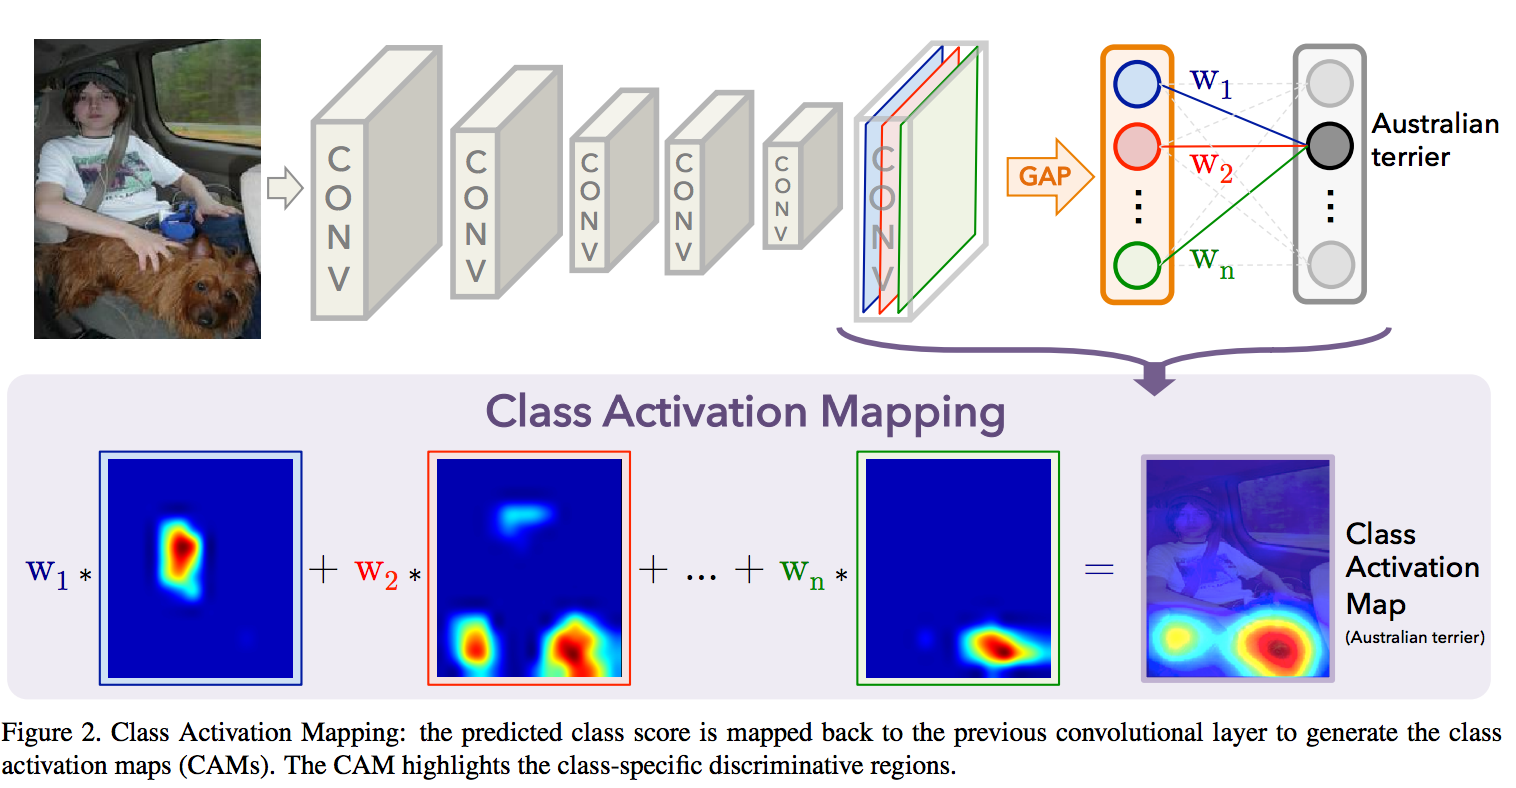
\includegraphics{https://raw.githubusercontent.com/FrancescoSaverioZuppichini/A-journey-into-Convolutional-Neural-Network-visualization-/master/resources/images/class_activation_mapping1.png}
\caption{alt}
\end{figure}

    By changing the target class, we can see different part of the image
highlighted. The first image uses the prediction class, while the second
\texttt{cat} and the last one \texttt{bookcase}, just to see what the
model will do with a wrong class.

    \begin{Verbatim}[commandchars=\\\{\}]
{\color{incolor}In [{\color{incolor}74}]:} \PY{k+kn}{from} \PY{n+nn}{visualisation}\PY{n+nn}{.}\PY{n+nn}{core}\PY{n+nn}{.}\PY{n+nn}{utils} \PY{k}{import} \PY{n}{imshow}
         
         \PY{n}{module} \PY{o}{=} \PY{n}{resnet34}\PY{p}{(}\PY{k+kc}{True}\PY{p}{)}
         \PY{n}{module}\PY{o}{.}\PY{n}{eval}\PY{p}{(}\PY{p}{)}
         
         \PY{n}{vis} \PY{o}{=} \PY{n}{ClassActivationMapping}\PY{p}{(}\PY{n}{module}\PY{p}{,} \PY{n}{device}\PY{p}{)}
         
         \PY{n}{classes} \PY{o}{=} \PY{p}{[}\PY{k+kc}{None}\PY{p}{,} \PY{l+m+mi}{285}\PY{p}{,} \PY{l+m+mi}{453}\PY{p}{]}
         
         \PY{k}{def} \PY{n+nf}{vis\PYZus{}outs2images\PYZus{}classes}\PY{p}{(}\PY{n}{outs}\PY{p}{)}\PY{p}{:}
             \PY{n}{images} \PY{o}{=} \PY{p}{[}\PY{n}{x}\PY{p}{[}\PY{l+m+mi}{0}\PY{p}{]} \PY{k}{for} \PY{n}{x} \PY{o+ow}{in} \PY{n}{outs}\PY{p}{]}
             \PY{n}{classes} \PY{o}{=} \PY{p}{[}\PY{n}{imagenet2human}\PY{p}{[}\PY{n+nb}{int}\PY{p}{(}\PY{n}{x}\PY{p}{[}\PY{l+m+mi}{1}\PY{p}{]}\PY{p}{[}\PY{l+s+s1}{\PYZsq{}}\PY{l+s+s1}{prediction}\PY{l+s+s1}{\PYZsq{}}\PY{p}{]}\PY{p}{)}\PY{p}{]} \PY{k}{for} \PY{n}{x} \PY{o+ow}{in} \PY{n}{outs}\PY{p}{]}
             
             \PY{k}{return} \PY{n}{images}\PY{p}{,} \PY{n}{classes}
         
         \PY{n}{outs} \PY{o}{=} \PY{p}{[}\PY{n}{vis}\PY{p}{(}\PY{n}{inputs}\PY{p}{[}\PY{l+m+mi}{0}\PY{p}{]}\PY{p}{,} \PY{k+kc}{None}\PY{p}{,} 
                   \PY{n}{postprocessing}\PY{o}{=}\PY{n}{image\PYZus{}net\PYZus{}postprocessing}\PY{p}{,} 
                   \PY{n}{target\PYZus{}class}\PY{o}{=}\PY{n}{c}\PY{p}{,}
                   \PY{n}{guide}\PY{o}{=}\PY{k+kc}{True}\PY{p}{)} \PY{k}{for} \PY{n}{c} \PY{o+ow}{in} \PY{n}{classes}\PY{p}{]}
         
         \PY{n}{images}\PY{p}{,} \PY{n}{classes} \PY{o}{=} \PY{n}{vis\PYZus{}outs2images\PYZus{}classes}\PY{p}{(}\PY{n}{outs}\PY{p}{)}
         
         \PY{n}{subplot}\PY{p}{(}\PY{n}{images}\PY{p}{,} 
                 \PY{n}{rows\PYZus{}titles}\PY{o}{=}\PY{n}{classes}\PY{p}{,}
                 \PY{n}{nrows}\PY{o}{=}\PY{l+m+mi}{1}\PY{p}{,} 
                 \PY{n}{ncols}\PY{o}{=}\PY{l+m+mi}{3}\PY{p}{,} 
                 \PY{n}{parse}\PY{o}{=}\PY{n}{tensor2img}\PY{p}{)}
\end{Verbatim}


    
    \begin{verbatim}
<IPython.core.display.Javascript object>
    \end{verbatim}

    
    
    \begin{verbatim}
<IPython.core.display.HTML object>
    \end{verbatim}

    
    Let's plot the CAM for the \texttt{cat} for different \texttt{resnet}
architecture. For resnet \textgreater{} 34 the \texttt{Bottleneck}
module is used

    \begin{Verbatim}[commandchars=\\\{\}]
{\color{incolor}In [{\color{incolor}76}]:} \PY{n}{modules\PYZus{}instances} \PY{o}{=} \PY{p}{[}\PY{n}{resnet18}\PY{p}{,} \PY{n}{resnet34}\PY{p}{,} \PY{n}{resnet101}\PY{p}{,} \PY{n}{resnet152}\PY{p}{]}
         
         \PY{n}{cat} \PY{o}{=} \PY{n}{inputs}\PY{p}{[}\PY{l+m+mi}{2}\PY{p}{]}
         
         \PY{n}{modules} \PY{o}{=} \PY{p}{(}\PY{n}{m}\PY{p}{(}\PY{n}{pretrained}\PY{o}{=}\PY{k+kc}{True}\PY{p}{)} \PY{k}{for} \PY{n}{m} \PY{o+ow}{in} \PY{n}{modules\PYZus{}instances}\PY{p}{)} \PY{c+c1}{\PYZsh{} make a generator, we don\PYZsq{}t want to store in memory all of them at once}
         
         \PY{n}{run\PYZus{}vis\PYZus{}plot\PYZus{}across\PYZus{}models}\PY{p}{(}\PY{n}{modules}\PY{p}{,} \PY{n}{cat}\PY{p}{,} \PY{k+kc}{None}\PY{p}{,} 
                                    \PY{n}{ClassActivationMapping} \PY{p}{,} 
                                    \PY{l+s+s1}{\PYZsq{}}\PY{l+s+s1}{ClassActivationMapping}\PY{l+s+s1}{\PYZsq{}}\PY{p}{,} 
                                    \PY{n}{nrows}\PY{o}{=}\PY{n+nb}{len}\PY{p}{(}\PY{n}{modules\PYZus{}instances}\PY{p}{)}\PY{p}{,}
                                    \PY{n}{ncols}\PY{o}{=}\PY{l+m+mi}{1}\PY{p}{,}
                                    \PY{n}{postprocessing}\PY{o}{=}\PY{n}{image\PYZus{}net\PYZus{}postprocessing}\PY{p}{,} 
                                    \PY{n}{rows\PYZus{}name} \PY{o}{=} \PY{p}{[}\PY{l+s+s1}{\PYZsq{}}\PY{l+s+s1}{resnet18}\PY{l+s+s1}{\PYZsq{}}\PY{p}{,} \PY{l+s+s1}{\PYZsq{}}\PY{l+s+s1}{resnet34}\PY{l+s+s1}{\PYZsq{}}\PY{p}{,} \PY{l+s+s1}{\PYZsq{}}\PY{l+s+s1}{resnet101}\PY{l+s+s1}{\PYZsq{}}\PY{p}{,} \PY{l+s+s1}{\PYZsq{}}\PY{l+s+s1}{resnet152}\PY{l+s+s1}{\PYZsq{}}\PY{p}{]}\PY{p}{,}
                                    \PY{n}{target\PYZus{}class}\PY{o}{=}\PY{k+kc}{None}\PY{p}{)}
\end{Verbatim}


    \begin{Verbatim}[commandchars=\\\{\}]
/usr/local/lib/python3.6/site-packages/matplotlib/pyplot.py:524: RuntimeWarning: More than 20 figures have been opened. Figures created through the pyplot interface (`matplotlib.pyplot.figure`) are retained until explicitly closed and may consume too much memory. (To control this warning, see the rcParam `figure.max\_open\_warning`).
  max\_open\_warning, RuntimeWarning)

    \end{Verbatim}

    
    \begin{verbatim}
<IPython.core.display.Javascript object>
    \end{verbatim}

    
    
    \begin{verbatim}
<IPython.core.display.HTML object>
    \end{verbatim}

    
    They are all very similar. \texttt{resnet101} is a little weird. One
huge problem with this visualisation is that it forced you to have a
specific architecture.

    \section{Grad Cam}\label{grad-cam}

    \textbf{Grad Cam} was introduced by
\href{https://arxiv.org/abs/1610.02391}{Grad-CAM: Visual Explanations
from Deep Networks via Gradient-based Localization}. The idea is
actually simple, we backprop the output with respect to a target class
while storing the gradient and the output at a given layer, in our case
the last convolution. Then we perform a global average of the saved
gradient keeping the channel dimension in order to get a 1-d tensor,
this will represent the importance of each channel in the target
convolutional layer. We then multiply each element of the convolutional
layer outputs by the averaged gradients to create the grad cam. This
whole procedure is fast and it is architecture independent. Interesting,
the authors show that is a generalization of the previous technique.

\begin{figure}
\centering
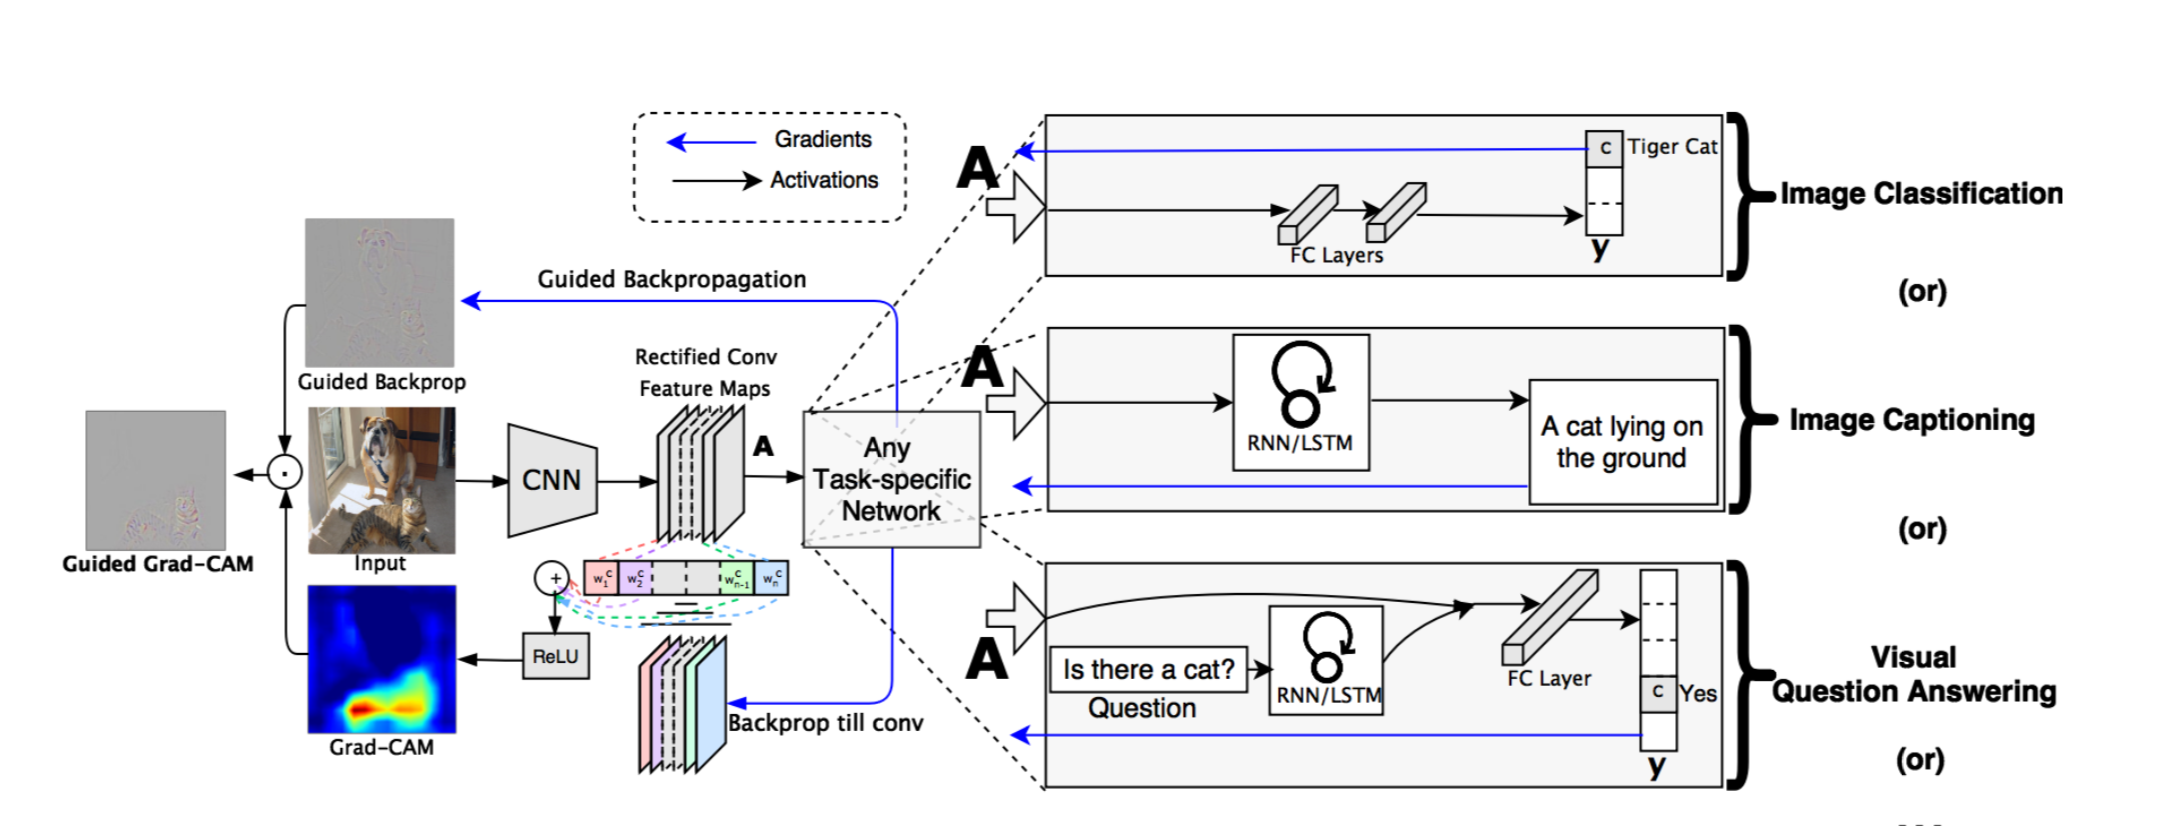
\includegraphics{https://raw.githubusercontent.com/FrancescoSaverioZuppichini/A-journey-into-Convolutional-Neural-Network-visualization-/master/resources/images/grad_cam1.png}
\caption{alt}
\end{figure}

    We can use it to higlight what different models are looking at.

    \begin{Verbatim}[commandchars=\\\{\}]
{\color{incolor}In [{\color{incolor}79}]:} \PY{n}{modules\PYZus{}instances} \PY{o}{=} \PY{p}{[}\PY{n}{alexnet}\PY{p}{,} \PY{n}{vgg16}\PY{p}{,} \PY{n}{resnet34}\PY{p}{]}
         
         \PY{n}{modules} \PY{o}{=} \PY{p}{(}\PY{n}{m}\PY{p}{(}\PY{n}{pretrained}\PY{o}{=}\PY{k+kc}{True}\PY{p}{)} \PY{k}{for} \PY{n}{m} \PY{o+ow}{in} \PY{n}{modules\PYZus{}instances}\PY{p}{)} \PY{c+c1}{\PYZsh{} make a generator, we don\PYZsq{}t want to store in memory all of them at once}
         
         
         \PY{n}{run\PYZus{}vis\PYZus{}plot\PYZus{}across\PYZus{}models}\PY{p}{(}\PY{n}{modules}\PY{p}{,} \PY{n}{inputs}\PY{p}{[}\PY{l+m+mi}{0}\PY{p}{]}\PY{p}{,} \PY{k+kc}{None}\PY{p}{,} \PY{n}{GradCam} \PY{p}{,} \PY{l+s+s1}{\PYZsq{}}\PY{l+s+s1}{Gradcam}\PY{l+s+s1}{\PYZsq{}}\PY{p}{,} 
                                    \PY{n}{nrows}\PY{o}{=}\PY{l+m+mi}{1}\PY{p}{,} 
                                    \PY{n}{ncols}\PY{o}{=}\PY{l+m+mi}{3}\PY{p}{,} 
                                    \PY{n}{target\PYZus{}class}\PY{o}{=}\PY{k+kc}{None}\PY{p}{,} 
                                    \PY{n}{postprocessing}\PY{o}{=}\PY{n}{image\PYZus{}net\PYZus{}postprocessing}\PY{p}{)}
\end{Verbatim}


    \begin{Verbatim}[commandchars=\\\{\}]
/usr/local/lib/python3.6/site-packages/matplotlib/pyplot.py:524: RuntimeWarning: More than 20 figures have been opened. Figures created through the pyplot interface (`matplotlib.pyplot.figure`) are retained until explicitly closed and may consume too much memory. (To control this warning, see the rcParam `figure.max\_open\_warning`).
  max\_open\_warning, RuntimeWarning)

    \end{Verbatim}

    
    \begin{verbatim}
<IPython.core.display.Javascript object>
    \end{verbatim}

    
    
    \begin{verbatim}
<IPython.core.display.HTML object>
    \end{verbatim}

    
    It is really interesting to see how Alexnet looks at the upper nose and
the eye, whiile vgg at the nose and restnet at the whole dog. We can
also others target classes as we did before.

    \begin{Verbatim}[commandchars=\\\{\}]
{\color{incolor}In [{\color{incolor}80}]:} \PY{k+kn}{from} \PY{n+nn}{visualisation}\PY{n+nn}{.}\PY{n+nn}{core}\PY{n+nn}{.}\PY{n+nn}{utils} \PY{k}{import} \PY{n}{imshow}
         
         \PY{n}{module} \PY{o}{=} \PY{n}{resnet34}\PY{p}{(}\PY{k+kc}{True}\PY{p}{)}
         \PY{n}{module}\PY{o}{.}\PY{n}{eval}\PY{p}{(}\PY{p}{)}
         
         \PY{n}{vis} \PY{o}{=} \PY{n}{GradCam}\PY{p}{(}\PY{n}{module}\PY{p}{,} \PY{n}{device}\PY{p}{)}
         
         \PY{n}{classes} \PY{o}{=} \PY{p}{[}\PY{k+kc}{None}\PY{p}{,} \PY{l+m+mi}{285}\PY{p}{,} \PY{l+m+mi}{453}\PY{p}{]}
         \PY{n}{outs} \PY{o}{=} \PY{p}{[}\PY{n}{vis}\PY{p}{(}\PY{n}{inputs}\PY{p}{[}\PY{l+m+mi}{0}\PY{p}{]}\PY{p}{,} \PY{k+kc}{None}\PY{p}{,} 
                   \PY{n}{postprocessing}\PY{o}{=}\PY{n}{image\PYZus{}net\PYZus{}postprocessing}\PY{p}{,} 
                   \PY{n}{target\PYZus{}class}\PY{o}{=}\PY{n}{c}\PY{p}{)} \PY{k}{for} \PY{n}{c} \PY{o+ow}{in} \PY{n}{classes}\PY{p}{]}
         
         \PY{n}{images}\PY{p}{,} \PY{n}{classes} \PY{o}{=} \PY{n}{vis\PYZus{}outs2images\PYZus{}classes}\PY{p}{(}\PY{n}{outs}\PY{p}{)}
         
         \PY{n}{subplot}\PY{p}{(}\PY{n}{images}\PY{p}{,}
                 \PY{n}{title}\PY{o}{=}\PY{l+s+s1}{\PYZsq{}}\PY{l+s+s1}{resnet34}\PY{l+s+s1}{\PYZsq{}}\PY{p}{,}
                 \PY{n}{rows\PYZus{}titles}\PY{o}{=}\PY{n}{classes}\PY{p}{,}
                 \PY{n}{nrows}\PY{o}{=}\PY{l+m+mi}{1}\PY{p}{,} 
                 \PY{n}{ncols}\PY{o}{=}\PY{n+nb}{len}\PY{p}{(}\PY{n}{outs}\PY{p}{)}\PY{p}{,} 
                 \PY{n}{parse}\PY{o}{=}\PY{n}{tensor2img}\PY{p}{)}
\end{Verbatim}


    \begin{Verbatim}[commandchars=\\\{\}]
/usr/local/lib/python3.6/site-packages/matplotlib/pyplot.py:524: RuntimeWarning: More than 20 figures have been opened. Figures created through the pyplot interface (`matplotlib.pyplot.figure`) are retained until explicitly closed and may consume too much memory. (To control this warning, see the rcParam `figure.max\_open\_warning`).
  max\_open\_warning, RuntimeWarning)

    \end{Verbatim}

    
    \begin{verbatim}
<IPython.core.display.Javascript object>
    \end{verbatim}

    
    
    \begin{verbatim}
<IPython.core.display.HTML object>
    \end{verbatim}

    
    We can now plot the grad cam for each input with respect to each model

    \begin{Verbatim}[commandchars=\\\{\}]
{\color{incolor}In [{\color{incolor}81}]:} \PY{n}{modules\PYZus{}instances} \PY{o}{=} \PY{p}{[}\PY{n}{alexnet}\PY{p}{,} \PY{n}{vgg16}\PY{p}{,} \PY{n}{resnet34}\PY{p}{,} \PY{n}{resnet152}\PY{p}{]}
         
         \PY{n}{modules} \PY{o}{=} \PY{p}{(}\PY{n}{m}\PY{p}{(}\PY{n}{pretrained}\PY{o}{=}\PY{k+kc}{True}\PY{p}{)} \PY{k}{for} \PY{n}{m} \PY{o+ow}{in} \PY{n}{modules\PYZus{}instances}\PY{p}{)} \PY{c+c1}{\PYZsh{} make a generator, we don\PYZsq{}t want to store in memory all of them at once}
         
         
         \PY{n}{run\PYZus{}vis\PYZus{}plot\PYZus{}across\PYZus{}models}\PY{p}{(}\PY{n}{modules}\PY{p}{,} \PY{n}{inputs}\PY{p}{[}\PY{l+m+mi}{0}\PY{p}{]}\PY{p}{,} \PY{k+kc}{None}\PY{p}{,} \PY{n}{GradCam} \PY{p}{,} \PY{l+s+s1}{\PYZsq{}}\PY{l+s+s1}{Gradcam}\PY{l+s+s1}{\PYZsq{}}\PY{p}{,} 
                                    \PY{n}{nrows}\PY{o}{=}\PY{l+m+mi}{4}\PY{p}{,} 
                                    \PY{n}{ncols}\PY{o}{=}\PY{l+m+mi}{3}\PY{p}{,} 
                                    \PY{n}{target\PYZus{}class}\PY{o}{=}\PY{k+kc}{None}\PY{p}{,} 
                                    \PY{n}{inputs}\PY{o}{=}\PY{n}{inputs}\PY{p}{,}
                                    \PY{n}{annotations}\PY{o}{=}\PY{p}{[}\PY{l+s+s1}{\PYZsq{}}\PY{l+s+s1}{alexnet}\PY{l+s+s1}{\PYZsq{}}\PY{p}{,} \PY{l+s+s1}{\PYZsq{}}\PY{l+s+s1}{vgg16}\PY{l+s+s1}{\PYZsq{}}\PY{p}{,} \PY{l+s+s1}{\PYZsq{}}\PY{l+s+s1}{resnet34}\PY{l+s+s1}{\PYZsq{}}\PY{p}{,} \PY{l+s+s1}{\PYZsq{}}\PY{l+s+s1}{resnet152}\PY{l+s+s1}{\PYZsq{}}\PY{p}{]}\PY{p}{,}
                                    \PY{n}{postprocessing}\PY{o}{=}\PY{n}{image\PYZus{}net\PYZus{}postprocessing}\PY{p}{)}
\end{Verbatim}


    \begin{Verbatim}[commandchars=\\\{\}]
/usr/local/lib/python3.6/site-packages/matplotlib/pyplot.py:524: RuntimeWarning: More than 20 figures have been opened. Figures created through the pyplot interface (`matplotlib.pyplot.figure`) are retained until explicitly closed and may consume too much memory. (To control this warning, see the rcParam `figure.max\_open\_warning`).
  max\_open\_warning, RuntimeWarning)

    \end{Verbatim}

    
    \begin{verbatim}
<IPython.core.display.Javascript object>
    \end{verbatim}

    
    
    \begin{verbatim}
<IPython.core.display.HTML object>
    \end{verbatim}

    
    Probably the most interesting column is the cat. \texttt{alexnet} looks
at some part of the face and the ears, while \texttt{vgg} uses only the
ears to tell that it is a cat. The two resnet models look at the whole
cat.

    We talk before about interesting region localizations. Grad-cam can be
also used to extract the class object out of the image. Easily, once the
have the grad-cam image we can used it as mask to crop out form the
input image what we want.

    \begin{Verbatim}[commandchars=\\\{\}]
{\color{incolor}In [{\color{incolor}82}]:} \PY{n}{model} \PY{o}{=} \PY{n}{resnet34}\PY{p}{(}\PY{k+kc}{True}\PY{p}{)}
         \PY{n}{model}\PY{o}{.}\PY{n}{eval}\PY{p}{(}\PY{p}{)}
         
         \PY{n}{vis} \PY{o}{=} \PY{n}{GradCam}\PY{p}{(}\PY{n}{model}\PY{p}{,} \PY{n}{device}\PY{p}{)}
         
         \PY{n}{\PYZus{}} \PY{o}{=} \PY{n}{vis}\PY{p}{(}\PY{n}{inputs}\PY{p}{[}\PY{l+m+mi}{0}\PY{p}{]}\PY{p}{,} \PY{k+kc}{None}\PY{p}{,} 
                   \PY{n}{postprocessing}\PY{o}{=}\PY{n}{image\PYZus{}net\PYZus{}postprocessing}\PY{p}{)}
\end{Verbatim}


    \begin{Verbatim}[commandchars=\\\{\}]
{\color{incolor}In [{\color{incolor}83}]:} \PY{k+kn}{import} \PY{n+nn}{cv2}
         
         \PY{k}{def} \PY{n+nf}{gradcam2crop}\PY{p}{(}\PY{n}{cam}\PY{p}{,} \PY{n}{original\PYZus{}img}\PY{p}{)}\PY{p}{:}
             \PY{n}{b}\PY{p}{,} \PY{n}{c}\PY{p}{,} \PY{n}{w}\PY{p}{,} \PY{n}{h} \PY{o}{=} \PY{n}{inputs}\PY{p}{[}\PY{l+m+mi}{0}\PY{p}{]}\PY{o}{.}\PY{n}{shape}
             \PY{n}{cam} \PY{o}{=} \PY{n}{cv2}\PY{o}{.}\PY{n}{resize}\PY{p}{(}\PY{n}{cam}\PY{o}{.}\PY{n}{numpy}\PY{p}{(}\PY{p}{)}\PY{p}{,} \PY{p}{(}\PY{n}{w}\PY{p}{,}\PY{n}{h}\PY{p}{)}\PY{p}{)}
             
             \PY{n}{mask} \PY{o}{=} \PY{n}{cam} \PY{o}{\PYZgt{}} \PY{l+m+mf}{0.7}
         
             \PY{n}{original\PYZus{}img} \PY{o}{=} \PY{n}{tensor2img}\PY{p}{(}\PY{n}{image\PYZus{}net\PYZus{}postprocessing}\PY{p}{(}\PY{n}{original\PYZus{}img}\PY{p}{[}\PY{l+m+mi}{0}\PY{p}{]}\PY{o}{.}\PY{n}{squeeze}\PY{p}{(}\PY{p}{)}\PY{p}{)}\PY{p}{)}
         
             \PY{n}{crop} \PY{o}{=} \PY{n}{original\PYZus{}img}\PY{o}{.}\PY{n}{copy}\PY{p}{(}\PY{p}{)}
             \PY{n}{crop}\PY{p}{[}\PY{n}{mask} \PY{o}{==} \PY{l+m+mi}{0}\PY{p}{]} \PY{o}{=} \PY{l+m+mi}{0}
             
             \PY{k}{return} \PY{n}{crop}
         
         \PY{n}{crop} \PY{o}{=} \PY{n}{gradcam2crop}\PY{p}{(}\PY{n}{vis}\PY{o}{.}\PY{n}{cam}\PY{p}{,} \PY{n}{inputs}\PY{p}{[}\PY{l+m+mi}{0}\PY{p}{]}\PY{p}{)}
         
         \PY{n}{fig} \PY{o}{=} \PY{n}{plt}\PY{o}{.}\PY{n}{figure}\PY{p}{(}\PY{p}{)}
         \PY{n}{plt}\PY{o}{.}\PY{n}{imshow}\PY{p}{(}\PY{n}{crop}\PY{p}{)}
\end{Verbatim}


    \begin{Verbatim}[commandchars=\\\{\}]
/usr/local/lib/python3.6/site-packages/matplotlib/pyplot.py:524: RuntimeWarning: More than 20 figures have been opened. Figures created through the pyplot interface (`matplotlib.pyplot.figure`) are retained until explicitly closed and may consume too much memory. (To control this warning, see the rcParam `figure.max\_open\_warning`).
  max\_open\_warning, RuntimeWarning)

    \end{Verbatim}

    
    \begin{verbatim}
<IPython.core.display.Javascript object>
    \end{verbatim}

    
    
    \begin{verbatim}
<IPython.core.display.HTML object>
    \end{verbatim}

    
\begin{Verbatim}[commandchars=\\\{\}]
{\color{outcolor}Out[{\color{outcolor}83}]:} <matplotlib.image.AxesImage at 0x1304a3160>
\end{Verbatim}
            
    \emph{et voilà}! We can also change again class, and crop the interest
region for that class.

    \begin{Verbatim}[commandchars=\\\{\}]
{\color{incolor}In [{\color{incolor}84}]:} \PY{n}{\PYZus{}} \PY{o}{=} \PY{n}{vis}\PY{p}{(}\PY{n}{inputs}\PY{p}{[}\PY{l+m+mi}{0}\PY{p}{]}\PY{p}{,} \PY{k+kc}{None}\PY{p}{,} 
                 \PY{n}{target\PYZus{}class}\PY{o}{=}\PY{l+m+mi}{282}\PY{p}{,}
                   \PY{n}{postprocessing}\PY{o}{=}\PY{n}{image\PYZus{}net\PYZus{}postprocessing}\PY{p}{)}
         
         \PY{n}{crop} \PY{o}{=} \PY{n}{gradcam2crop}\PY{p}{(}\PY{n}{vis}\PY{o}{.}\PY{n}{cam}\PY{p}{,} \PY{n}{inputs}\PY{p}{[}\PY{l+m+mi}{0}\PY{p}{]}\PY{p}{)}
         
         \PY{n}{fig} \PY{o}{=} \PY{n}{plt}\PY{o}{.}\PY{n}{figure}\PY{p}{(}\PY{p}{)}
         \PY{n}{plt}\PY{o}{.}\PY{n}{imshow}\PY{p}{(}\PY{n}{crop}\PY{p}{)}
\end{Verbatim}


    \begin{Verbatim}[commandchars=\\\{\}]
/usr/local/lib/python3.6/site-packages/matplotlib/pyplot.py:524: RuntimeWarning: More than 20 figures have been opened. Figures created through the pyplot interface (`matplotlib.pyplot.figure`) are retained until explicitly closed and may consume too much memory. (To control this warning, see the rcParam `figure.max\_open\_warning`).
  max\_open\_warning, RuntimeWarning)

    \end{Verbatim}

    
    \begin{verbatim}
<IPython.core.display.Javascript object>
    \end{verbatim}

    
    
    \begin{verbatim}
<IPython.core.display.HTML object>
    \end{verbatim}

    
\begin{Verbatim}[commandchars=\\\{\}]
{\color{outcolor}Out[{\color{outcolor}84}]:} <matplotlib.image.AxesImage at 0x12fc1ada0>
\end{Verbatim}
            
    \subsection{Different models}\label{different-models}

    We have seen all these techniques used with classic classicification
models trained on \texttt{imagenet}. What about use them on a different
domain? I have ported this paper to Pytorch and retrain it. The model
learn from the frontal camera's image of a robot to predict the local
distance sensors in order to avoid obstacles. Let's see what if, by
using those techniques, we can understand better what is going on inside
the model.


    % Add a bibliography block to the postdoc
    
    
    
    \end{document}
